 \documentclass{magnolia}

\magtex{tex_driver={pdftex},
        tex_packages={epigraph,xypic,tikz,pgfplots,nicefrac}}
\magfiche{document_nom={Cours sur les probabilités},
          auteur_nom={François Fayard},
          auteur_mail={francois.fayard@auxlazaristeslasalle.fr}}
\magcours{cours_matiere={maths},
          cours_niveau={mpsi},
          cours_chapitre_numero={20},
          cours_chapitre={Probabilités}}
\magmisenpage{misenpage_presentation={tikzvelvia},
              misenpage_format={a4},
              misenpage_nbcolonnes={1},
              misenpage_preuve={non},
              misenpage_sol={non}}
\magmisenpage{}
\maglieudiff{}
\magprocess

\begin{document}
%BEGIN_BOOK

% - La probabilté uniforme arrive tard. Mettre plus haut
% - Les justifications sur les probabilités "naturelles" sont souvent "pipo"
%   Il faut expliquer quelles probabilités mettre



\setlength\epigraphwidth{.7\textwidth}
\epigraph{\og Il y a tellement de gens qui trouvent à travers le monde la seule femme qu'ils puissent aimer, que l'énorme fréquence de ces rencontres me rend sceptique, moi qui ai un certain respect du calcul des probabilités. \fg}{--- {\sc Tristan Bernard (1866--1947)}}
\hidemesometimes{
\hfill\includegraphics[width=0.5\textwidth]{../../Commun/Images/maths-cours-conditional_risk.png}}

\magtoc

\section{Espace probabilisé}

La théorie des probabilités est la modélisation mathématique des phénomènes caractérisés par
le hasard et l'incertitude. Considérons par exemple le jeu de \og pile ou face \fg.
Avant d'effectuer un lancer, nous savons que le résultat de cette expérience sera soit
pile, soit face. Il est impossible de prévoir le résultat d'un unique lancer, mais si nous effectuons $n$ lancers et que
nous comptons le nombre $n_P$ de fois où on a obtenu pile, on constate que la proportion
$n_P/n$ tend vers \nicefrac{1}{2} lorsque $n$ tend vers l'infini.

\begin{center}
    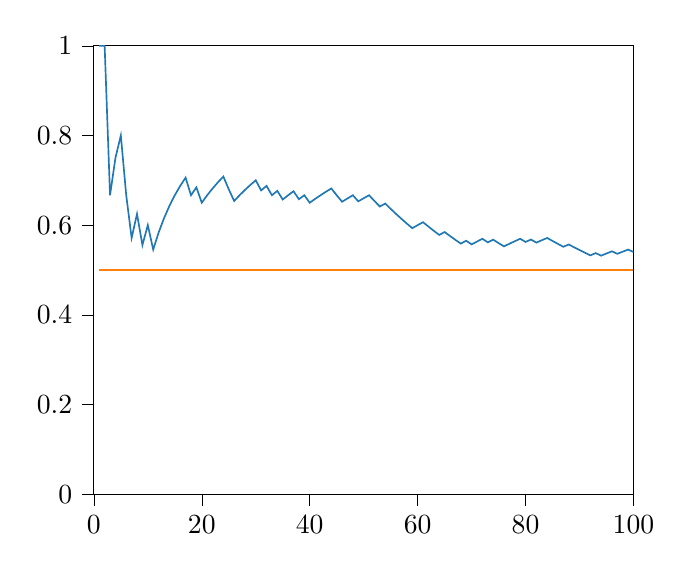
\begin{tikzpicture}
    
            \definecolor{color0}{rgb}{0.12156862745098,0.466666666666667,0.705882352941177}
            \definecolor{color1}{rgb}{1,0.498039215686275,0.0549019607843137}
            
            \begin{axis}[
            tick align=outside,
            tick pos=left,
            x grid style={white!69.0196078431373!black},
            xmin=0, xmax=100,
            xtick style={color=black},
            y grid style={white!69.0196078431373!black},
            ymin=0.0, ymax=1.0,
            ytick style={color=black}
            ]
            \addplot [semithick, color0]
            table {%
            1 1
            2 1
            3 0.666666666666667
            4 0.75
            5 0.8
            6 0.666666666666667
            7 0.571428571428571
            8 0.625
            9 0.555555555555556
            10 0.6
            11 0.545454545454545
            12 0.583333333333333
            13 0.615384615384615
            14 0.642857142857143
            15 0.666666666666667
            16 0.6875
            17 0.705882352941177
            18 0.666666666666667
            19 0.684210526315789
            20 0.65
            21 0.666666666666667
            22 0.681818181818182
            23 0.695652173913043
            24 0.708333333333333
            25 0.68
            26 0.653846153846154
            27 0.666666666666667
            28 0.678571428571429
            29 0.689655172413793
            30 0.7
            31 0.67741935483871
            32 0.6875
            33 0.666666666666667
            34 0.676470588235294
            35 0.657142857142857
            36 0.666666666666667
            37 0.675675675675676
            38 0.657894736842105
            39 0.666666666666667
            40 0.65
            41 0.658536585365854
            42 0.666666666666667
            43 0.674418604651163
            44 0.681818181818182
            45 0.666666666666667
            46 0.652173913043478
            47 0.659574468085106
            48 0.666666666666667
            49 0.653061224489796
            50 0.66
            51 0.666666666666667
            52 0.653846153846154
            53 0.641509433962264
            54 0.648148148148148
            55 0.636363636363636
            56 0.625
            57 0.614035087719298
            58 0.603448275862069
            59 0.593220338983051
            60 0.6
            61 0.60655737704918
            62 0.596774193548387
            63 0.587301587301587
            64 0.578125
            65 0.584615384615385
            66 0.575757575757576
            67 0.567164179104478
            68 0.558823529411765
            69 0.565217391304348
            70 0.557142857142857
            71 0.563380281690141
            72 0.569444444444444
            73 0.561643835616438
            74 0.567567567567568
            75 0.56
            76 0.552631578947368
            77 0.558441558441558
            78 0.564102564102564
            79 0.569620253164557
            80 0.5625
            81 0.567901234567901
            82 0.560975609756098
            83 0.566265060240964
            84 0.571428571428571
            85 0.564705882352941
            86 0.558139534883721
            87 0.551724137931034
            88 0.556818181818182
            89 0.550561797752809
            90 0.544444444444444
            91 0.538461538461538
            92 0.532608695652174
            93 0.537634408602151
            94 0.531914893617021
            95 0.536842105263158
            96 0.541666666666667
            97 0.536082474226804
            98 0.540816326530612
            99 0.545454545454545
            100 0.54
            };
            \addplot [semithick, color1]
            table {%
            1 0.5
            2 0.5
            3 0.5
            4 0.5
            5 0.5
            6 0.5
            7 0.5
            8 0.5
            9 0.5
            10 0.5
            11 0.5
            12 0.5
            13 0.5
            14 0.5
            15 0.5
            16 0.5
            17 0.5
            18 0.5
            19 0.5
            20 0.5
            21 0.5
            22 0.5
            23 0.5
            24 0.5
            25 0.5
            26 0.5
            27 0.5
            28 0.5
            29 0.5
            30 0.5
            31 0.5
            32 0.5
            33 0.5
            34 0.5
            35 0.5
            36 0.5
            37 0.5
            38 0.5
            39 0.5
            40 0.5
            41 0.5
            42 0.5
            43 0.5
            44 0.5
            45 0.5
            46 0.5
            47 0.5
            48 0.5
            49 0.5
            50 0.5
            51 0.5
            52 0.5
            53 0.5
            54 0.5
            55 0.5
            56 0.5
            57 0.5
            58 0.5
            59 0.5
            60 0.5
            61 0.5
            62 0.5
            63 0.5
            64 0.5
            65 0.5
            66 0.5
            67 0.5
            68 0.5
            69 0.5
            70 0.5
            71 0.5
            72 0.5
            73 0.5
            74 0.5
            75 0.5
            76 0.5
            77 0.5
            78 0.5
            79 0.5
            80 0.5
            81 0.5
            82 0.5
            83 0.5
            84 0.5
            85 0.5
            86 0.5
            87 0.5
            88 0.5
            89 0.5
            90 0.5
            91 0.5
            92 0.5
            93 0.5
            94 0.5
            95 0.5
            96 0.5
            97 0.5
            98 0.5
            99 0.5
            100 0.5
            };
            \end{axis}
            
            \end{tikzpicture}
    \end{center}
\noindent
En mathématiques, nous modélisons cette expérience en disant que l'univers des possibles est un
ensemble $\Omega\defeq\ens{P, F}$ formé de deux éléments  et que la probabilité de l'évènement
$A\defeq\ens{P}$ est \nicefrac{1}{2}, ce que l'on note
\[\mathbb{P}(\ens{P})=\frac{1}{2}.\]
Puisque le nombre $n_F$ de fois où on a obtenu face vérifie $n_P+n_F=n$, on en déduit que
la probabilité d'obtenir face est aussi de \nicefrac{1}{2}, ce que l'on note de même
$\mathbb{P}(\ens{F})=1/2$.\\

Considérons maintenant un autre jeu de hasard~: le lancer d'un dé à 6 faces. Dans ce cas,
l'univers des possibles est $\Omega\defeq\intere{1}{6}$. On constate que quel que
soit $\omega\in\Omega$, si on lance le dé $n$ fois et qu'on compte le nombre $n_\omega$ de
fois où on a obtenu $\omega$, la proportion $n_\omega/n$ tend vers $\nicefrac{1}{6}$. On écrira
\[\forall \omega\in\intere{1}{6}\qsep \mathbb{P}(\ens{\omega})=\frac{1}{6}.\]
Si l'on s'intéresse au nombre $n_P$ de fois où on a obtenu un nombre pair, c'est-à-dire au
nombre de fois où on a obtenu 2, 4 ou 6, nous dirons que nous nous intéressons à l'évènement
$A\defeq\ens{2,4,6}$. Bien entendu
\[\frac{n_P}{n}=\frac{n_2+n_4+n_6}{n}=\frac{n_2}{n}+\frac{n_4}{n}+\frac{n_6}{n}
  \tendvers{n}{+\infty} 3\times\frac{1}{6}=\frac{1}{2}.\]
On écrira 
\[\mathbb{P}(\ens{2, 4, 6})=\frac{1}{2}.\]
Nous remarquons que sur ces deux exemples, l'univers $\Omega$ est fini et que, quelle que soit
la partie $A$ de $\Omega$, on a
\[\mathbb{P}(A)=\frac{\card A}{\card \Omega}.\]
Nous dirons que la probabilité $\mathbb{P}$ est uniforme sur $\Omega$.\\

Cependant, les probabilités ne sont pas toujours uniformes. On considère par exemple
l'expérience
qui consiste à avoir 2 enfants. Si on s'intéresse au sexe des enfants, il y a trois
possibilités~: on peut avoir deux filles, deux garçons ou une fille et un garçon. Nous
modélisons cela en disant que l'univers des possibles est $\Omega\defeq\ens{F,G,D}$.
L'expérience montre que la probabilité d'avoir deux filles est de $\nicefrac{1}{4}$,
celle d'avoir deux garçons est de $\nicefrac{1}{4}$ et celle d'avoir une fille et un
garçon est de $\nicefrac{1}{2}$. Nous avons donc un exemple simple où la
probabilité n'est pas uniforme.\\

En 1881, l'astronome
\nom{Simon Newcomb} se rend compte que les livres de tables de logarithmes sont plus
abimés à certaines pages qu'à d'autres. Sa découverte suggère que les personnes
ayant besoin de faire des applications numériques sont plus souvent confrontées à des nombres
commençant par un 1, comme 1491 ou $1.602\times 10^{-19}$, que par un 9, comme $987$ ou $9.81$.
Soixante ans plus tard, \nom{Frank Benford}, après avoir
répertorié un très grand nombre de données, dont les longueurs des fleuves et les populations
des villes, fait le même constat. Ici, l'univers des possibles est $\Omega\defeq\intere{1}{9}$
et \nom{Benford} postule que
\[\forall \omega\in\intere{1}{9}\qsep \mathbb{P}(\ens{\omega})=\log_{10}\p{1+\frac{1}{\omega}}.\]

\begin{center}
% This file was created by tikzplotlib v0.9.8.
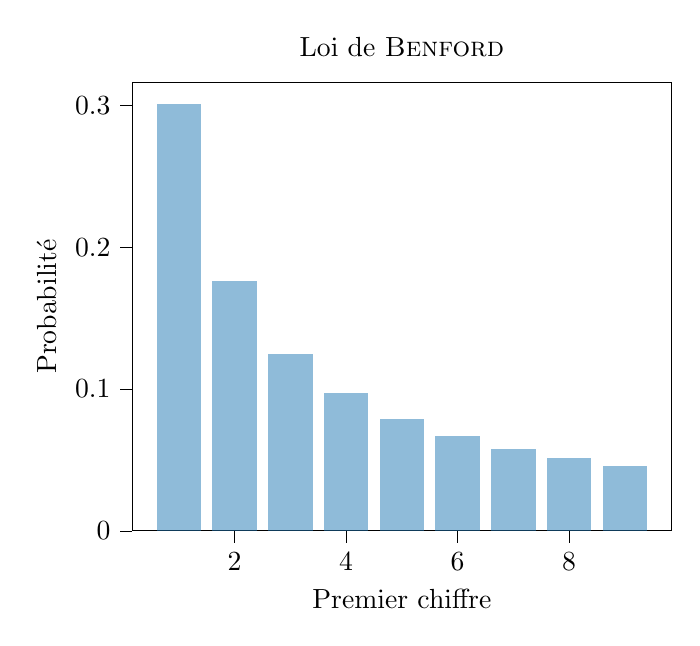
\begin{tikzpicture}

\definecolor{color0}{rgb}{0.12156862745098,0.466666666666667,0.705882352941177}

\begin{axis}[
tick align=outside,
tick pos=left,
title={Loi de \textsc{Benford}},
x grid style={white!69.0196078431373!black},
xlabel={Premier chiffre},
xmin=0.16, xmax=9.84,
xtick style={color=black},
y grid style={white!69.0196078431373!black},
ylabel={Probabilité},
ymin=0, ymax=0.31608149544718,
ytick style={color=black}
]
\draw[draw=none,fill=color0,fill opacity=0.5] (axis cs:0.6,0) rectangle (axis cs:1.4,0.301029995663981);
\draw[draw=none,fill=color0,fill opacity=0.5] (axis cs:1.6,0) rectangle (axis cs:2.4,0.176091259055681);
\draw[draw=none,fill=color0,fill opacity=0.5] (axis cs:2.6,0) rectangle (axis cs:3.4,0.1249387366083);
\draw[draw=none,fill=color0,fill opacity=0.5] (axis cs:3.6,0) rectangle (axis cs:4.4,0.0969100130080564);
\draw[draw=none,fill=color0,fill opacity=0.5] (axis cs:4.6,0) rectangle (axis cs:5.4,0.0791812460476248);
\draw[draw=none,fill=color0,fill opacity=0.5] (axis cs:5.6,0) rectangle (axis cs:6.4,0.0669467896306132);
\draw[draw=none,fill=color0,fill opacity=0.5] (axis cs:6.6,0) rectangle (axis cs:7.4,0.0579919469776867);
\draw[draw=none,fill=color0,fill opacity=0.5] (axis cs:7.6,0) rectangle (axis cs:8.4,0.0511525224473813);
\draw[draw=none,fill=color0,fill opacity=0.5] (axis cs:8.6,0) rectangle (axis cs:9.4,0.0457574905606751);
\end{axis}

\end{tikzpicture}

\end{center}
\noindent
On vérifie que
\begin{eqnarray*}
\sum_{\omega=1}^9 \mathbb{P}(\ens{\omega})
&=& \sum_{\omega=1}^9 \log_{10}\p{1+\frac{1}{\omega}}
= \sum_{\omega=1}^9 \cro{\log_{10}\p{\omega+1}-\log_{10}\p{\omega}}\\
&=& \log_{10}\p{10}-\log_{10}\p{1} = 1
\end{eqnarray*}
comme attendu pour une probabilité.

\subsection{Espace probabilisé}

\begin{definition}
Étant donné une expérience aléatoire, on appelle \emph{univers des possibles} ou simplement
\emph{univers} tout ensemble fini $\Omega$ où chaque élément $\omega\in\Omega$ représente une
\emph{réalisation} de l'expérience.
\end{definition}

\begin{exemples}
\exemple \emph{Série de Pile ou Face}. Soit $n\in\N$. On considère l'expérience aléatoire
  qui consiste à jeter $n$ fois une pièce. Dans ce cas, l'univers des possibles est
  $\Omega\defeq\ens{P,F}^n$, la lettre $P$ représentant le résultat pile et la lettre
  $F$ représentant le résultat face. Par exemple, si $n=3$,
  $\omega\defeq(P,P,F)$ représente la réalisation de l'expérience où les deux premiers
   lancers donnent pile et le dernier lancer donne face.
\exemple \emph{Répartition de $n$ boules discernables dans $p$ urnes discernables}. Soit
  $n,p\in\N$. On considère l'expérience qui consiste à répartir de manière aléatoire $n$
  boules discernables dans $p$ urnes discernables. On choisit de numéroter les boules de
  1 à $n$ et les urnes de $1$ à $p$. L'univers des possibles est donc
  $\Omega_D\defeq\intere{1}{p}^n$ et une réalisation $\omega\in\Omega$ de l'expérience
   est un $n$-uplet $(\omega_1,\ldots,\omega_n)$ où pour tout $i\in\intere{1}{n}$,
  $\omega_i\in\intere{1}{p}$ est le numéro de l'urne dans laquelle on a placé la boule $i$.
\exemple
  \emph{Répartition de $n$ boules indiscernables dans $p$ urnes discernables}. Soit
  $n,p\in\N$. On considère l'expérience qui consiste à répartir de manière aléatoire
  $n$ boules indiscernables dans $p$ urnes discernables. Une réalisation est
  caractérisée par le nombre de boules $x_1,\ldots,x_p\in\N$ que contient chaque urne.
  Comme on sait qu'il y a au total $n$ boules, l'univers des possibles est donc
  \[\Omega_I\defeq\enstq{(x_1,\ldots,x_p)\in\N^p}{x_1+\cdots+x_p=n}.\]
\end{exemples}

\begin{remarqueUnique}
\remarque En première année, l'univers des possibles sera toujours un ensemble fini. Cette
  restriction nous empêchera de modéliser certaines expériences comme jouer à pile ou face
  jusqu'à obtenir pile. La théorie des probabilités sur un univers infini est
  plus délicate. C'est pourquoi vous ne l'aborderez qu'en seconde année.
\end{remarqueUnique}

\begin{definition}
Soit $\Omega$ l'univers des possibles.
\begin{itemize}
\item On appelle \emph{évènement} toute partie de $\Omega$. L'évènement $\Omega$ est appelé
  \emph{évènement certain} et l'évènement $\emptyset$ est appelé \emph{évènement impossible}.
\item On dit que deux évènements $A,B\in\mathcal{P}(\Omega)$ sont
  \emph{disjoints}, ou \emph{incompatibles}, lorsque
  $A\cap B=\emptyset$.
\end{itemize}
\end{definition}

\begin{remarques}
\remarque On dit que les évènements $A_1,\ldots,A_n\in\mathcal{P}(\Omega)$ sont incompatibles
  lorsque
  \[\forall i,j\in\intere{1}{n}\qsep i\neq j\implique A_i\cap A_j=\emptyset.\]
\remarque On dit qu'un évènement $A$ est \emph{élémentaire} lorsqu'il ne contient qu'un résultat
  observable, c'est-à-dire lorsqu'il existe $\omega\in\Omega$ tel que $A=\ens{\omega}$.
\remarque Si $A$ et $B\in\mathcal{P}(\Omega)$ sont des évènements, on appelle
  \begin{itemize}
  \item évènement \og $A$ et $B$ \fg l'évènement $A\cap B$.
  \item évènement \og $A$ ou $B$ \fg l'évènement $A\cup B$.
  \item évènement \og contraire de $A$ \fg l'évènement $\bar{A}=\Omega\setminus A$.
  \end{itemize}
\end{remarques}


\begin{exoUnique}
\exo On considère l'expérience consistant à jeter $n$ fois une pièce.
  Pour tout $k\in\intere{1}{n}$, on considère l'évènement
  $F_k\defeq$ \og Le résultat du $k$-ième lancer est face \fg. Exprimer, en fonction des $F_k$,
  les évènements suivants~:
  \begin{itemize}
  \item $A\defeq$ \og On n'obtient jamais pile au cours des $n$ lancers \fg.
  \item $B\defeq$ \og On obtient pile au moins une fois au cours au cours des $n$ lancers\fg.
  \item $C\defeq$ \og On obtient deux faces consécutifs au cours des $n$ lancers \fg.
  \end{itemize}

\end{exoUnique}

% \begin{exos}
% \exo Soit $A_1,\dots,A_n$ des évènements sur un univers $\Omega$. Exprimer en fonction des
%   $A_i$ les évènements suivants.
%   \begin{itemize}
%   \item $A \defeq$ \og Tous les $A_i$ sont réalisés \fg.
%   \item $B \defeq$ \og L'un des $A_i$ est réalisé \fg.
%   \item $C \defeq$ \og Aucun des $A_i$ n'est réalisé \fg.
%   \item $D \defeq$ \og Au moins l'un des $A_i$ n'est pas réalisé \fg.
%   \item $E \defeq$ \og Un seul des $A_i$ est réalisé \fg.
%   \end{itemize}
% \begin{sol}
% \begin{enumerate}
% \item $\bigcap_{i=1}^n A_i$.
% \item $\bigcup_{i=1}^n A_i$.
% \item $\overline{\bigcup_{i=1}^n A_i}$.
% \item $\bigcup_{i=1}^n \overline{A_i}$.
% \item $\bigcup_{i=1}^n \p{(\cap_{j\neq i}^n \overline{A_j})\cap A_i}$. 
% \end{enumerate}
% \end{sol}
% \exo On tire au hasard deux cartes dans un jeu de 32 cartes
%   (as, roi, dame, valet, 10, 9, 8, 7). On considère les évènements suivants.
%   \begin{itemize}
%   \item $A \defeq$ \og les deux cartes tirées sont rouges \fg
%   \item $B \defeq$ \og les deux cartes tirées sont un valet et un dix \fg
%   \item $C \defeq$ \og les deux cartes tirées sont des personnages \fg
%   \end{itemize}
%   Décrire par des phrases les évènements suivants.
%   \[\bar{A},\quad A \cap B \cap \bar{C},\quad A \cap B \cap C\]
% \begin{sol}
% "Au moins une des cartes n'est pas rouge". "Une carte est un valet rouge et l'autre est un 10 rouge". "C'est l'évènement impossible donc on peut dire n'importe quelle phrase impossible".
% \end{sol}
% \end{exos}
  

\begin{definition}
Soit $\Omega$ l'univers des possibles. On dit que la famille d'évènements
$(A_1,\ldots,A_n)\in\mathcal{P}(\Omega)^n$ forme un \emph{système complet d'évènements}
lorsque c'est une partition de $\Omega$, c'est-à-dire lorsque
\[\Omega = \bigcup_{i=1}^n A_i \qquad\et\qquad \cro{\forall i,j\in\intere{1}{n}\qsep i\neq j\implique
  A_i\cap A_j=\emptyset}.\]
\end{definition}


% \begin{exemples}
% \exemple Dans un casino, il y a $n$ machines à sous. On choisit une machine au hasard et on
%   joue une fois sur cette machine ce qui nous donne soit gagnant, soit perdant.
%   Dans ce cas, l'univers des possibles est
%   $\Omega\defeq\intere{1}{n}\times\ens{g, p}$. Par exemple, un résultat observable de cette
%   expérience est $\omega\defeq(3,g)$; il signifie qu'un a choisi la machine 3 et qu'on a
%   gagné. Pour tout $k\in\intere{1}{n}$, on note $M_k$ l'évènement \og on a choisi la
%   $k$-ième machine \fg. D'autre part, on note $G$ l'évènement \og on a gagné \fg et $P$
%   l'évènement \og on a perdu\fg. Alors $(G,P)$ forme un système complet d'évènements. De
%   même, $(M_1,\ldots,M_n)$ forme un système complet d'évènements
% \end{exemples}

\begin{definition}
On appelle \emph{loi de probabilité}, \emph{mesure de probabilité} ou plus simplement \emph{probabilité} sur un univers $\Omega$
toute application
\[\dspappli{\mathbb{P}}{\mathcal{P}(\Omega)}{\interf{0}{1}}{A}{\mathbb{P}(A)}\]
telle que
\begin{itemize}
\item $\mathbb{P}(\Omega)=1$
\item $\forall A,B\in\mathcal{P}(\Omega)\qsep A\cap B=\emptyset \quad\implique\quad
  \mathbb{P}(A\cup B)=\mathbb{P}(A)+\mathbb{P}(B)$.
\end{itemize}
Le couple $(\Omega,\mathbb{P})$ est appelé \emph{espace probabilisé}.
\end{definition}

\begin{remarqueUnique}
\remarque On dit que deux évènements $A$ et $B$ sont \emph{équiprobables}
  lorsque $\mathbb{P}(A)=\mathbb{P}(B)$.
% \remarque Si $\Omega$ est un ensemble fini non vide, l'application $\mathbb{P}$ définie par
% \[\forall A\in\mathcal{P}(\Omega)\qsep \mathbb{P}(A)=\frac{\card A}{\card \Omega}.\]  
% est une probabilité que nous appelerons \emph{probabilité uniforme}.
\end{remarqueUnique}

\begin{definition}
  Soit $\Omega$ un ensemble fini non vide. On appelle \emph{probabilité uniforme} sur $\Omega$
  l'application $\mathbb{P}:\mathcal{P}(\Omega)\to\interf{0}{1}$ définie par
  \[\forall A\in\mathcal{P}(\Omega)\qsep \mathbb{P}(A)=\frac{\card A}{\card \Omega}.\] 
  \end{definition}
  
  \begin{remarques}
  % \remarque Cherchons à déterminer les probabilités \og naturelles \fg sur les 3 exemples que nous avons
  %   donnés en début de cours.
  \remarque Lorsque $\Omega$ est muni d'une loi uniforme, les calculs de probabilité se ramènent à des
    problèmes de dénombrement.
\remarque Pour deux des trois exemples d'expérience aléatoire que nous avons donné
  en début de cours, la probabilité \og naturelle \fg
  est la probabilité uniforme.
    \begin{itemize}
    \item \emph{Série de Pile ou Face}~: Si on considère l'expérience aléatoire qui consiste à jeter $n$ fois une
      pièce équilibrée, c'est la  probabilité uniforme qui est naturelle sur l'univers $\Omega\defeq\ens{P,F}^n$. Nous montrerons plus tard que cela
      revient à supposer que les
      résultats de chaque lancer ont autant de chance de donner pile que face, et que les lancers sont indépendants.
    \item \emph{Répartition de $n$ boules discernables dans $p$ urnes discernables}~: Si l'on souhaite répartir
      $n$ boules discernables dans $p$ urnes discernables, c'est encore la
      probabilité uniforme qui est naturelle sur $\Omega_D\defeq\intere{1}{p}^n$. Nous verrons que cela revient à supposer que chaque
      boule est placée de manière équiprobable dans les différentes urnes et que ces répartitions sont indépendantes les unes
      des autres.
    % \item \emph{Répartition de $n$ boules indiscernables dans $p$ urnes discernables}~: Enfin, si l'expérience
    %   est de répartir $n$ boules indiscernables dans $p$ urnes discernables, la probabilité naturelle n'est
    %   plus la probabilité uniforme. Pour s'en convaincre, on peut essayer de comprendre ce qui se passe pour
    %   $n=2$ et $p=2$. On considère donc l'expérience qui consiste à placer deux boules indiscernables dans 2 urnes
    %   distinctes. Il y a 3 réalisations possibles de cette expérience~: \og Les deux boules sont dans la première urne \fg,
    %   \og Les deux boules sont dans la seconde urne\fg et \og Il y a une boule dans chaque urne\fg. L'univers des possibles
    %   $\Omega_I$ possède donc 3 éléments. On se convaincra facilement que l'évènement \og Il y a une boule dans
    %   chaque urne \fg a une probabilité naturelle de \nicefrac{1}{2}. En effet, une fois que la première boule est placée,
    %   on a une chance sur deux que la seconde boule soit placée dans la même urne. Les probabilités naturelles
    %   pour cette expérience sont donc respectivement de \nicefrac{1}{4}, \nicefrac{1}{4} et \nicefrac{1}{2}, ce
    %   qui ne dérive pas d'une loi uniforme. Pour traiter ce type de problème, on peut considérer que
    %   les boules sont discernables et travailler sur $\Omega_D$ muni de la probabilité uniforme.
    \end{itemize}
  \end{remarques}

Dans la suite de ce cours, $(\Omega,\mathbb{P})$ désignera un espace probabilisé.

\begin{proposition}
\begin{eqnarray*}
\mathbb{P}(\emptyset)=0,& &\mathbb{P}(\Omega)=1,\\
\forall A\in\mathcal{P}(\Omega),& &\mathbb{P}(\bar{A})=1-\mathbb{P}(A),\\
\forall A,B\in\mathcal{P}(\Omega),& &\mathbb{P}(A\cup B)=\mathbb{P}(A)+\mathbb{P}(B)-\mathbb{P}(A\cap B).
\end{eqnarray*}
\end{proposition}

\begin{proposition}
Une probabilité est une fonction \emph{croissante}. Autrement dit
\[\forall A,B\in\mathcal{P}(\Omega)\qsep A\subset B \quad\implique\quad \mathbb{P}(A)\leq\mathbb{P}(B).\]
\end{proposition}

\begin{proposition}
Soit $(A_1,\ldots,A_n)\in\mathcal{P}(\Omega)^n$ une famille d'évènements incompatibles.
Alors
\[\mathbb{P}\p{\bigcup_{i=1}^n A_i}=\sum_{i=1}^n \mathbb{P}(A_i).\]
\end{proposition}

\begin{remarques}
\remarque Si $A_1,\ldots,A_n$ est une famille d'évènements incompatibles, la réunion des $A_i$ est parfois
  notée
  \[\bigsqcup_{i=1}^n A_i.\]
\remarque Si $A_1,\ldots,A_n$ sont quelconques, on a seulement
  \[\mathbb{P}\p{\bigcup_{i=1}^n A_i}\leq\sum_{i=1}^n \mathbb{P}(A_i).\]
  On dit que $\mathbb{P}$ est \emph{sous-additive}. 
\end{remarques}

\begin{exos}
  \exo Une urne contient 20 boules, numérotées de 1 à 20~: 5 boules sont blanches,
  5 sont rouges et 10 sont noires.
  On tire successivement 3 boules, avec remise à chaque tirage.
  Si on munit $\Omega$ de la probabilité uniforme,
  calculer la probabilité que
    le tirage soit~:
    \begin{itemize}
  \item unicolore.
  \item tricolore.
  \item bicolore.
    \end{itemize}
  % \question On tire 3 boules simultanément. Reprendre les questions précédentes.
  % \end{questions}
  \begin{sol}
  \begin{questions}
  \question $\Card\Omega=20^3=8000$~: ce sont des triplets de $\intere{1}{20}$. La loi de probabilité est uniforme.
    \begin{itemize}
    \item $\Card A=10\times 5\time 5\times 3!$. On trouve une probabilité de $3/16$.
    \item $\Card B=375+375+1500+750+1500+750$. On troube une proba de $21/32$.
    \item $\Card C=125+!25+1000$. On trouve une proba de $5/32$.
    \end{itemize}
  \question $\Card\Omega=\binom{20}{3}=1440$.
    \begin{itemize}
    \item $250$, puis $25/114$.
<    \item $25/38$.
    \item $7/57$.
    \end{itemize}
  \end{questions}
  \end{sol}
  \exo Une urne contient 8 boules, numérotées de 1 à 8~: 3 boules sont blanches et
    5 sont noires. On en tire simultanément 4 boules.
    Si on munit $\Omega$ de la probabilité uniforme, avec quelle probabilité
    n'a-t-on tiré que des boules noires~?
    \begin{sol}
    On trouve (4 parmi 5)/(4 parmi 8) et donc \nicefrac{1}{14}.
    \end{sol}
\end{exos}

\begin{proposition}[nom={Formule du crible}]
Soit $(A_1,\ldots,A_n)\in\mathcal{P}(\Omega)^n$ une famille d'évènements. Alors
  \[\mathbb{P}\p{\bigcup_{i=1}^n A_i}=\sum_{k=1}^n (-1)^{k+1}
    \sum_{1\leq i_1<\cdots<i_k\leq n}
    \mathbb{P}\p{A_{i_1}\cap\cdots\cap A_{i_k}}.\]
\end{proposition}

\begin{remarqueUnique}
\remarque   Par exemple, pour $n=3$, la formule du crible s'écrit
\[\mathbb{P}\p{A_1\cup A_2\cup A_3}=\mathbb{P}(A_1)+\mathbb{P}(A_2)+\mathbb{P}(A_3) - \cro{\mathbb{P}(A_2\cap A_3)+\mathbb{P}(A_1\cap A_3)+\mathbb{P}(A_1\cap A_2)}+\mathbb{P}(A_1\cap A_2\cap A_3).\]
\end{remarqueUnique}


\begin{definition}
\begin{itemize}
\item On appelle \emph{distribution de probabilité} sur
  $\Omega$ toute famille $(p_{\omega})_{\omega\in\Omega}$ de réels positifs telle que
  \[\sum_{\omega\in\Omega} p_{\omega}=1.\]
\item Si $\mathbb{P}$ est une probabilité sur $\Omega$, on appelle \emph{distribution de
  probabilité} de $\mathbb{P}$ la famille $(p_{\omega})_{\omega\in\Omega}$ définie par
  \[\forall \omega\in\Omega\qsep p_{\omega}\defeq \mathbb{P}(\ens{\omega}).\]
  C'est une distribution de probabilité sur $\Omega$.
\end{itemize}
\end{definition}

% \begin{remarqueUnique}
% \remarque Si $(p_\omega)_{\omega\in\Omega}$ est une distribution de probabilité sur $\Omega$, on appelle support
%   de $p$ l'ensemble $\enstq{\omega\in\Omega}{p_{\omega}>0}$.
%   Par extension, le support d'une probabilité $\mathbb{P}$ est le support de sa distribution de probabilité.
%   Autrement dit
%   \[{\rm Supp}(\mathbb{P})\defeq\enstq{\omega\in\Omega}{\mathbb{P}(\ens{\omega})>0}.\]
%   % On s'intéressera le plus souvent à des espaces probabilisés $(\Omega,\mathbb{P})$
%   % pour lesquels ${\rm Supp}(\mathbb{P})=\Omega$.
% \end{remarqueUnique}
\begin{remarqueUnique}
  \remarque Si $\mathbb{P}$ désigne la probabilité uniforme sur l'univers $\Omega$ de cardinal $n$, alors
quel que soit $\omega\in\Omega$, $p_\omega=1/n$.
\end{remarqueUnique}

\begin{exoUnique}
\exo Sur l'univers $\Omega\defeq\intere{0}{n}$, on définit la famille $(p_k)_{0\leq k\leq n}$ par
  \[\forall k\in\intere{0}{n}\qsep p_k\defeq\alpha\binom{n}{k}\]
  où $\alpha\in\R$. Déterminer $\alpha$ pour que $(p_k)_{0\leq k\leq n}$ soit une distribution de probabilité. 
\end{exoUnique}


\begin{proposition}
Soit $(\Omega,\mathbb{P})$ un espace probabilisé et $(p_\omega)_{\omega\in\Omega}$ la distribution de probabilité de $\mathbb{P}$. Alors
\[\forall A\in\mathcal{P}(\Omega)\qsep \mathbb{P}(A)=\sum_{\omega\in A} p_{\omega}.\]
\end{proposition}

\begin{remarques}
\remarque Une probabilité est donc entièrement déterminée par sa distribution de probabilité.
% \remarque 
  % Un évènement $A$ est presque sûr si et seulement si ${\rm Supp}(\mathbb{P})\subset A$.
% \remarque En particulier, deux probabilités $\mathbb{P}_1$ et $\mathbb{P}_2$, définies sur un même univers
%   $\Omega$, sont égales si et seulement si
%   \[\forall \omega\in\Omega\qsep \mathbb{P}_1(\ens{\omega})=\mathbb{P}_2(\ens{\omega}).\]
\remarque Une probabilité est donc uniforme si et seulement si tous les évènements élémentaires sont équiprobables.
Une erreur très classique en probabilités est de croire que la mesure de probabilité \og naturelle \fg
sur un univers est toujours la probabilité uniforme. Ce n'est pas toujours le cas. Cependant, lorsque ça l'est,
un argument de symétrie permet souvent de s'en convaincre.
Par exemple, si on lance un dé à 6 faces, les symétries du dé font que les valeurs obtenues sont
équiprobables. La mesure de probabilité \og naturelle \fg sur $\Omega\defeq\intere{1}{6}$ est donc la probabilité
uniforme.
\end{remarques}

\begin{exoUnique}
\exo On lance un dé pipé à 6 faces qui donne \og 1 \fg avec la probabilité \nicefrac{1}{4} et les
  autres faces avec une même probabilité $p$. Quelle est la probabilité d'obtenir un nombre impair~?
  \begin{sol}
  On trouve $p=3/20$, et $\mathbb{P}(Impair)=11/20$.
  \end{sol}
\end{exoUnique}

\begin{proposition}
Soit $(p_\omega)_{\omega\in\Omega}$ une distribution de probabilité sur l'univers $\Omega$. Alors il existe une
unique probabilité $\mathbb{P}$ sur $\Omega$ telle que
\[\forall \omega\in\Omega\qsep \mathbb{P}(\ens{\omega})=p_{\omega}.\]
\end{proposition}

% \begin{remarques}
% \remarque On considère l'expérience aléatoire qui consiste à lancer une pièce. L'univers
%   des possibles est $\Omega\defeq\ens{P,F}$, la lettre $P$ représentant le résultat pile,
%   et la lettre $F$ représentant le résultat face. Si la pièce est équilibrée, l'expérience
%   montre que la probabilité d'obtenir une pile est de \nicefrac{1}{2} et la probabilité
%   d'obtenir un face est de \nicefrac{1}{2}. C'est bien la probabilité
%   uniforme sur $\Omega$. 
% \remarque On considère l'expérience aléatoire qui consiste à lancer un dé à 6 faces.
%   L'univers des possibles est $\Omega\defeq\intere{1}{6}$. Si le dé n'est pas pipé,
%   l'expérience montre que quel que soit $\omega\in\intere{1}{6}$, la probabilité d'obtenir
%   $\omega$ est de \nicefrac{1}{6}. La probabilité naturelle sur $\Omega$ est donc la
%   probabilité uniforme.
% \remarque Soit $n\in\N$. On considère l'expérience aléatoire qui consiste à lancer $n$
%   fois une pièce. L'univers des possibles est donc $\Omega\defeq\ens{P,F}^n$.
%   En supposant que la probabilité d'obtenir un pile à chaque lancer est de \nicefrac{1}{2} et
%   que les lancers sont mutuellements indépendants, nous démontrerons plus tard que tous les
%   résultats sont équiprobables. La probabilité naturelle sur $\Omega$ est donc la probabilité
%   uniforme.
% \remarque Soit $n,p\in\N$. On considère l'expérience aléatoire qui consiste à placer $n$
%   boules discernables dans $p$ urnes discernables. En numérotant les boules de 1 à $n$ et
%   les urnes de 1 à $p$, l'univers des possibles est
%   $\Omega\defeq\mathcal{F}(\intere{1}{n},\intere{1}{p})$, un résultat observable étant une
%   application $\omega\in\Omega$ qui a une boule $i\in\intere{1}{n}$ associe l'urne $\omega(i)\in\intere{1}{p}$
%   dans laquelle elle a été placée. En supposant que les boules sont placées les unes
%   après les autres avec une probabilité uniforme sur toutes les urnes et qu'elle sont placées
%   de manière indépendante, nous démontrerons plus tard que tous les résultats sont
%   équiprobables. La probabilité naturelle sur $\Omega$ est donc la probabilité
%   uniforme.
% \end{remarques}

% \begin{proposition}
% Soit $\Omega=\ens{\omega_1,\ldots,\omega_n}$ un ensemble fini de cardinal $n$ et
% $p_1,\ldots,p_n\in\RP$ tels que $p_1+\cdots+p_n=1$. Alors il existe une unique
% mesure de probabiblité $\mathbb{P}$ sur $\Omega$ telle que
% \[\forall i\in\intere{1}{n}\qsep \mathbb{P}(\ens{\omega_i})=p_i.\]
% \end{proposition}



% \begin{definition}
% Soit $(\Omega,\mathbb{P})$ un espace probabilisé, $\Omega'$ un ensemble fini et
% $f:\Omega\to\Omega'$. Alors l'application
% \[\dspappli{\mathbb{P}_f}{\mathcal{P}(\Omega')}{\interf{0}{1}}{A}{\mathbb{P}\p{f^{-1}(A)}}\]
% est une probabilité sur $\Omega'$, appelée \emph{mesure image} de $\mathbb{P}$ par $f$.
% \end{definition}



% Ici, il faut parler de boules discernables et indiscernables.

% \begin{remarqueUnique}
% \remarque Soit $n,p\in\N$. On considère l'expérience aléatoire qui consiste à placer $n$
%   boules indiscernables dans $p$ urnes discernables. On note $\Omega$ l'univers des
%   possibles. Pour définir une probabilité
%   naturelle sur $\Omega$, il est bon de commencer par imaginer que les boules sont
%   discernables. Cela nous conduit à considérer l'univers $\Omega_1\defeq\mathcal{F}(\intere{1}{n},\intere{1}{p})$
%   muni de la probabilité uniforme $\mathbb{P}_1$. 
%   %  En numérotant les boules de 1 à $n$ et
%   % les urnes de 1 à $p$, l'univers des possibles est
%   % $\Omega\defeq\mathcal{F}(\intere{1}{n},\intere{1}{p})$, un résultat observable étant une
%   % application $\omega\in\Omega$ qui a une boule $i\in\intere{1}{n}$ associe l'urne $\omega(i)\in\intere{1}{p}$
%   % dans laquelle elle a été placée. En supposant que les boules sont placées les unes
%   % après les autres avec une probabilité uniforme sur toutes les urnes et qu'elle sont placées
%   % de manière indépendante, nous démontrerons plus tard que tous les résultats sont
%   % équiprobables. La probabilité naturelle sur $\Omega$ est donc la probabilité
%   % uniforme.
% \end{remarqueUnique}

\subsection{Variable aléatoire}

\begin{definition}
Soit $(\Omega,\mathbb{P})$ un espace probabilisé. On appelle \emph{variable aléatoire}
à valeurs dans $E$ toute application $X:\Omega\to E$.
\end{definition}

\begin{remarqueUnique}
\remarque On dit qu'une variable aléatoire $X:\Omega\to E$ est réelle lorsque $E$ est une
  partie de $\R$.
% \remarque Puisque $\Omega$ est fini, $X(\Omega)$ est fini. Si $E'$ est une partie finie de $E$
%   telle que $X(\Omega)\subset E'$, on se permettra de confondre $X$ et sa corestriction
%   à $E'$. On pourra donc se ramener au cas où $E$ est fini.
\end{remarqueUnique}

\begin{definition}
Soit $X:\Omega\to E$ une variable aléatoire. Alors, pour toute partie $A$ de $E$, on définit
l'évènement
\[(X\in A)\defeq\enstq{\omega\in\Omega}{X(\omega)\in A}.\] 
\end{definition}

\begin{remarques}
\remarque Si $x\in E$, l'évènement $\enstq{\omega\in\Omega}{X(\omega)=x}$ est noté
  $(X=x)$.
\remarque Si $X$ est une variable aléatoire réelle et $a,b\in\R$, l'évènement
  $\enstq{\omega\in\Omega}{a\leq X(\omega)\leq b}$ est noté $(a\leq X\leq b)$. 
\remarque L'évènement $(X\in A)$ est aussi noté $\ens{X\in A}$ ou $[X\in A]$. La probabilité
  d'un tel évènement est notée $\mathbb{P}(X\in A)$.
\end{remarques}

\begin{proposition}
Soit $X:\Omega\to E$ une variable aléatoire et $A,B\in\mathcal{P}(E)$. Alors
\[(X\in A\cap B)=(X\in A)\cap(X\in B), \qquad (X\in A\cup B)=(X\in A)\cup(X\in B),\]
\[(X\in \bar{A})=\overline{(X\in A)}.\]
\end{proposition}

\begin{exoUnique}
\exo Soit $X:\Omega\to\Z$ une variable aléatoire à valeurs entières. Montrer que
  \[\forall n\in\Z\qsep \mathbb{P}(X=n)=\mathbb{P}(X\leq n) - \mathbb{P}(X\leq n-1).\]
% \exo Soit $X$ une variable aléatoire réelle. Montrer que
%   $\mathbb{P}(X\leq 1)\leq \mathbb{P}(\abs{X-2}\geq 1)$.
% \exo On joue $n\in\Ns$ fois à pile ou face avec une pièce équilibrée. On compte le nombre
%   de lancers nécessaires $X$ pour obtenir pile pour la première fois. Si on obtient que des
%   faces, on pose $X=n+1$.
%   \begin{questions}
%   \question Modéliser l'expérience en précisant l'univers des possibles $\Omega$ et donner
%     une probabilité naturelle sur $\Omega$.
%   \question Pour tout $k\in\intere{0}{n}$, calculer $\mathbb{P}(X>k)$.
%   \question En déduire $\mathbb{P}(X=k)$ pour tout $k\in\intere{1}{n+1}$.
%   \end{questions}
\end{exoUnique}


\begin{definition}
Soit $X:\Omega\to E$ une variable aléatoire. Alors l'application
\[\dspappli{\mathbb{P}_X}{\mathcal{P}(X(\Omega))}{\interf{0}{1}}{A}{\mathbb{P}\p{X\in A}}\]
est une probabilité sur $X(\Omega)$, appelée \emph{loi} de $X$.
\end{definition}

\begin{remarques}
\remarque La loi de $X$ est entièrement déterminée par
  sa distribution de probabilité $(\mathbb{P}(X=x))_{x\in X(\Omega)}$.
\remarque Si $x\in E$ n'appartient pas à $X(\Omega)$, alors $\mathbb{P}(X=x)=0$.
\remarque 
  En pratique, lorsqu'il nous sera demandé de déterminer la loi d'une variable aléatoire
  $X:\Omega\to E$, on commencera par déterminer un ensemble fini $E'$ tel que $X(\Omega)\subset E'$
  puis on calculera $\mathbb{P}(X=x)$ pour tout $x\in E'$.
\remarque Si $(\Omega_1,\mathbb{P}_1)$ est un espace probabilisé, $\Omega_2$ est un ensemble fini et
  $F$ est une application de $\Omega_1$ dans $\Omega_2$, alors
  \[\dspappli{\mathbb{P}_2}{\mathcal{P}(\Omega_2)}{\interf{0}{1}}{A}{\mathbb{P}_1\p{F\in A}}\] 
  est une probabilité sur $\Omega_2$, appelée \emph{mesure image} de $\mathbb{P}_1$ par $F$.
\remarque
  En reprenant les notations utilisées dans les exemples de répartition de $n$ boules  
  discernables/indiscernables
  dans $p$ urnes discernables donnés plus haut, 
  on considère la fonction d'oubli $F:\Omega_D\to\Omega_I$. À une répartition de boules numérotées et donc discernables, elle associe
  la répartition
  des boules indiscernables, où on a effacé le numéro des boules. Autrement dit, si
  $\omega\defeq(\omega_1,\ldots,\omega_n)\in\Omega_D$, alors
  $F(\omega)=(x_1,\ldots,x_p)\in\Omega_I$ où
  \[\forall j\in\intere{1}{p}\qsep x_j=\card\enstq{i\in\intere{1}{n}}{\omega_i=j}.\]
La mesure de probabilité naturelle sur $\Omega_I$ est la mesure image par $F$ de la probabilité uniforme sur
  $\Omega_D$.
\end{remarques}

% \begin{remarques}
% % \remarque Le \emph{support de la variable aléatoire $X$} est défini comme étant le support
% %   de $\mathbb{P}_X$. Autrement dit
% %   \[{\rm Supp}(X)\defeq\enstq{x\in E}{\mathbb{P}(X=x)>0}.\]
% %   Remarquons que ${\rm Supp}(X)\subset X(\Omega)$, l'inclusion pouvant être stricte.
% \remarque Si l'on souhaite définir la loi d'une variable aléatoire $X:\Omega\to E$ à
%   valeurs dans un ensemble infini $E$, il suffit de considérer la corestriction
%   de $X$ à l'ensemble fini $E'\defeq X(\Omega)$. Étant donné que la détermination
%   exacte de $X(\Omega)$ nécessite parfois de traiter de nombreux
%   cas particuliers, nous nous contenterons de corestreindre $X$ à un ensemble fini $E'$ tel
%   que $X(\Omega)\subset E'$. Par exemple, si
%   $A\in\mathcal{P}(\Omega)$ et $X:\Omega\to\R$ est la fonction indicatrice
%   \[\dspappli{X}{\Omega}{\R}{\omega}{
%   \begin{cases}
%   1 & \text{si $\omega\in A$}\\
%   0 & \text{si $\omega\not\in A$.}
%   \end{cases}}\]
%   Alors $X(\Omega)\subset\ens{0,1}$. Cette inclusion est une égalité, sauf dans les cas
%   particuliers où $A=\emptyset$ et $A=\Omega$, pour lesquels $X(\Omega)$ est
%   respectivement égal à $\ens{0}$ et à $\ens{1}$. Pour une telle variable aléatoire,
%   on choisit $E'\defeq\ens{0,1}$. La distribution de probabilité $(p_0,p_1)$ de
%   $\mathbb{P}_X$ est alors donnée par
%   \[p_0=1-\mathbb{P}(A) \et p_1=\mathbb{P}(A).\]
%   Le plus souvent, on confondra $E'$ et $X(\Omega)$ et on écrira abusivement
%   $X(\Omega)=\ens{0,1}$.

% \end{remarques}

\begin{exoUnique}
\exo On lance successivement deux dés à 6 faces. On modélise cette expérience en choisissant $\Omega\defeq\intere{1}{6}^2$
  muni de la probabilité uniforme. On note $A_1:\Omega\to\N$ le résultat du premier dé et
  $A_2:\Omega\to\N$ le résultat du second dé. Déterminer les lois de $A_1$, $A_2$ ainsi que
  la loi de la variable aléatoire $A_1+A_2:\Omega\to\N$ donnant la somme des deux nombres
  obtenus.
\end{exoUnique}


% \begin{remarqueUnique}
  % Pour s'en convaincre, on considère l'expérience aléatoire qui consiste à jouer 2
  % fois à pile ou face. On modèlise cette expérience en posant $\Omega\defeq\ens{P,F}^2$ que
  % l'on munit de la probabilité uniforme. Soit $X_1:\Omega\to\ens{P,F}$ et
  % $X_2:\Omega\to\ens{P,F}$ les variables aléatoires donnant respectivement les résultats des
  % premiers et seconds lancers.  Alors $X_1$ et $X_2$ suivent la même loi. Pourtant, elles ne
  % sont pas égales.
% \end{remarqueUnique}

  
\begin{proposition}
Soit $X:\Omega\to E$ une variable aléatoire. Alors, pour toute partie $A$ de $E$
  \[\mathbb{P}(X\in A)=\sum_{x\in A} \mathbb{P}(X=x)\]
\end{proposition}

\begin{remarqueUnique}
\remarque Étant donné que $\mathbb{P}(X=x)$ est nul pour tout $x$ en dehors de l'ensemble
  fini $X(\Omega)$, cette somme est bien définie puisqu'elle ne comporte qu'un nombre fini
  de termes non nuls.
\end{remarqueUnique}


\begin{definition}
On dit que deux variables aléatoires $X,Y:\Omega\to E$ suivent la même
loi lorsque
\[\forall A\in\mathcal{P}(E)\qsep \mathbb{P}(X\in A)=\mathbb{P}(Y\in A).\]
Si tel est le cas, on écrit $X\sim Y$.
\end{definition}

\begin{remarques}
\remarque En pratique, pour montrer que $X$ et $Y$ suivent la même loi, il suffit de déterminer
  un ensemble fini $E'$ tel que $X(\Omega)\subset E'$ et $Y(\Omega)\subset E'$, puis de
  montrer que
  \[\forall a\in E'\qsep \mathbb{P}(X=a)=\mathbb{P}(Y=a).\]
\remarque Deux variables aléatoires qui suivent la même loi sont rarement égales.
  Par exemple, si $A$ est un évènement de probabilité \nicefrac{1}{2}, les variables
  aléatoires $\mathds{1}_A$ et $\mathds{1}_{\bar{A}}$ suivent la même loi sans être
  égales.
\end{remarques}

\begin{proposition}
Si $X:\Omega\to E$ une variable aléatoire, $X(\Omega)$ est un ensemble fini que l'on
note $\ens{x_1,\ldots,x_n}$. Alors, la famille des $(X=x_i)$ pour $i\in\intere{1}{n}$ forme
un système complet d'évènements.
\end{proposition}

\begin{remarques}
\remarque On utilisera souvent ce système complet d'évènements dans la formule des
  probabilités totales.
\remarque Cette proposition reste vraie si on remplace $X(\Omega)$ par une partie finie
  $E'$ de $E$ telle que $X(\Omega)\subset E'$.
\end{remarques}


\begin{definition}
Soit $X:\Omega\to E$ une variable aléatoire et $f:E\to F$. On note $f(X)$ la variable
aléatoire $f\circ X:\Omega\to F$.
\end{definition}

% \begin{proposition}

% \end{proposition}

% \begin{remarqueUnique}
% \remarque
 
% cette formule restant vraie si l'on remplace $X(\Omega)$ par une partie finie $E'$ de $E$
% telle que $X(\Omega)\subset E'$.
% \end{remarqueUnique}

\begin{remarqueUnique}
\remarque Soit $X:\Omega\to E$ une variable aléatoire et $f:E\to F$. Alors, pour tout
$y\in F$
\[\mathbb{P}(f(X)=y)=\sum_{x\in f^{-1}(\ens{y})} \mathbb{P}(X=x)\] 
  % \remarque Étant donné que $\mathbb{P}(X=x)$ est nul pour tout $x$ en dehors de l'ensemble
  %   fini $X(\Omega)$, cette somme est bien définie puisqu'elle ne comporte qu'un nombre fini
  %   de termes non nuls.
  \end{remarqueUnique}

\begin{proposition}
Soit $X,Y:\Omega\to E$ deux variables aléatoires et $f:E\to F$. Si $X\sim Y$, alors
$f(X)\sim f(Y)$.
\end{proposition}



\subsection{Lois usuelles}

% \begin{definition}[nom={Variable aléatoire constante}]
% On dit qu'une variable aléatoire $X:\Omega\to E$ est \emph{constante} lorsqu'il existe $a\in E$ tel
% que
% \[\mathbb{P}(X=a)=1.\]
% \end{definition}

% \begin{remarques}
% % \remarque Si $X:\Omega\to E$ est une variable aléatoire constante, il existe un unique
% %   $a\in E$ tel que $\mathbb{P}(X=a)=1$; on dit que $X$ est une variable aléatoire
% %   constante égale à $a$.
% % \remarque Une variable aléatoire $X:\Omega\to E$ est constante égale à $a\in E$, si et
% %   seulement si il existe un évènement presque sûr $A$ tel que
% %   \[\forall\omega\in A\qsep X(\omega)=a.\]
% \remarque Si $X:\Omega\to E$ est constante égale à $a$, alors
%   \[\forall x\in E\qsep \mathbb{P}(X=x)=
%   \begin{cases}
%   1 & \text{si $x=a$,}\\
%   0 & \text{sinon.}
%   \end{cases}\]
%   En particulier, ${\rm Supp}(\mathbb{P}_X)=\ens{a}$. On écrira parfois abusivement $X(\Omega)=\ens{a}$.
% \remarque Une variable aléatoire $X:\Omega\to E$ est constante si et seulement si il existe $a\in E$ et
%   un évènement presque sûr $A$ tel que
%   \[\forall \omega\in A\qsep X(\omega)=a.\]
% \end{remarques}


\begin{definition}[nom={Loi uniforme}]
Soit $A$ un ensemble fini non vide. On dit qu'une variable aléatoire $X$ à valeurs dans $A$
suit une \emph{loi uniforme} sur $A$ lorsque
\[\forall a\in A\qsep \mathbb{P}(X=a)=\frac{1}{\card A}.\]
Si tel est le cas, on note $X\sim\mathcal{U}(A)$.
\end{definition}

\begin{remarqueUnique}
\remarque Si $X$ suit une loi uniforme sur $A$, alors $X(\Omega)=A$.
\end{remarqueUnique}
% \begin{remarqueUnique}
% \remarque $X:\Omega\to A$ suit une loi uniforme sur $A$
% %   si et seulement si $\mathbb{P}_X$ est la probabilité uniforme sur $A$.
% \remarque Si $X:\Omega\to E$ suit une loi uniforme sur $A$, alors
%   \[\forall x\in E\qsep \mathbb{P}(X=x)=
%   \begin{cases}
%   \frac{1}{\card A} & \text{si $x\in A$,}\\
%   0 & \text{sinon.}
%   \end{cases}\]
%   En particulier, ${\rm Supp}(\mathbb{P}_X)=A$. On écrira parfois abusivement $X(\Omega)=A$.
% \end{remarqueUnique}
% \vspace{1ex}
\begin{exoUnique}
\exo Soit $X$ une variable aléatoire suivant une loi uniforme sur $\intere{-2}{2}$. Déterminer la loi
  de $X^2+1$.
\end{exoUnique}


\begin{definition}[nom={Loi de \nom{Bernoulli}}]
Soit $p\in[0,1]$. On dit qu'une variable aléatoire $X$ à valeurs dans $\ens{0,1}$ suit la \emph{loi de
\nom{Bernoulli}} de paramètre $p$ lorsque
\[\mathbb{P}(X=1)=p.\]
Si tel est le cas, $\mathbb{P}(X=0)=1-p$ et on note $X\sim\mathcal{B}(p)$.
\end{definition}

\begin{remarques}
\remarque Si $p\in[0,1]$, il est courant de poser $q\defeq 1-p\in[0,1]$.
% \remarque On a ${\rm Supp}(\mathbb{P}_X)\subset\ens{0,1}$, cette inclusion étant une
%   égalité si et seulement si $p\in]0,1[$.
%   On écrira parfois abusivement $X(\Omega)=\ens{0,1}$.
\remarque Si $X$ suit une loi de Bernoulli de paramètre $p\in]0,1[$, alors $X(\Omega)=\ens{0,1}$.
\remarque Toute variable aléatoire $X$ à valeurs dans $\ens{0,1}$ suit une loi de \nom{Bernoulli}
  de paramètre $p\defeq\mathbb{P}(X=1)$. En particulier, si $A\in\mathcal{P}(\Omega)$ est un évènement,
  alors $\mathds{1}_A$ est une variable aléatoire qui suit une
  loi de \nom{Bernoulli} de paramètre $p\defeq\mathbb{P}(A)$.
% \remarque Une loi de $\nom{Bernoulli}$ est constante si et seulement si $p=0$ ou $p=1$.
\remarque On dit qu'une variable aléatoire $Y$ à valeurs dans $\ens{-1,1}$ suit une loi de
  \nom{Rademacher} lorsque
  \[\mathbb{P}(Y=-1)=\frac{1}{2} \quad\et\quad \mathbb{P}(Y=1)=\frac{1}{2}.\]
  % Une variable aléatoire $Y$ suit une loi de \nom{Rademacher} si et seulement si il existe
  % une variable aléatoire $X$ suivant une loi de \nom{Bernoulli} de paramètre \nicefrac{1}{2}
  % telle que $Y=-1+2X$.
\end{remarques}

\begin{exempleUnique}
\exemple On considère l'expérience aléatoire d'un tir de penalty dans un match de foot. 
  La variable aléatoire $X:\Omega\to\ens{0,1}$ décrit le résultat de ce tir~: 1 si le
  penalty est réussi et 0 si le penalty est manqué. $X$ suit donc une loi de
  \nom{Bernoulli} dont le paramètre $p$ est estimé, selon les joueurs, entre $70\%$ et $90\%$.
\end{exempleUnique}

\begin{definition}[nom={Loi binomiale}]
Soit $n\in\N$ et $p\in[0,1]$. On dit qu'une variable aléatoire $X$ à valeurs dans $\intere{0}{n}$
suit la \emph{loi binomiale} de paramètre $(n,p)$ lorsque
\[\forall k\in\intere{0}{n}\qsep \mathbb{P}(X=k)=\binom{n}{k}p^k(1-p)^{n-k}.\]
Si tel est le cas, on note $X\sim\mathcal{B}(n,p)$. 
\end{definition}

\begin{remarques}
\remarque La loi binomiale $\mathcal{B}(1,p)$ n'est autre
  que la loi de \nom{Bernoulli} de paramètre $p$.
% \remarque On a ${\rm Supp}(\mathbb{P}_X)\subset\intere{0}{n}$, cette inclusion étant une
%   égalité si et seulement si $p\in ]0,1[$.
%   On écrira parfois abusivement $X(\Omega)=\intere{0}{n}$.
\remarque Si $X$ suit une loi binomiale de paramètre $(n,p)$ où $p\in]0,1[$, alors $X(\Omega)=\intere{0}{n}$.
\end{remarques}


% from scipy.special import binom
% import matplotlib.pyplot as plt
% import tikzplotlib as tikz
% n = 10
% p = 0.2
% r = [binom(n, k) * p**k * (1-p)**(n-k) for k in range(n)]
% plt.bar(range(n), r, alpha=0.5)
% tikz.save('/Users/fayard/Desktop/binomial-10.tex')

\begin{center}
% This file was created by tikzplotlib v0.9.8.
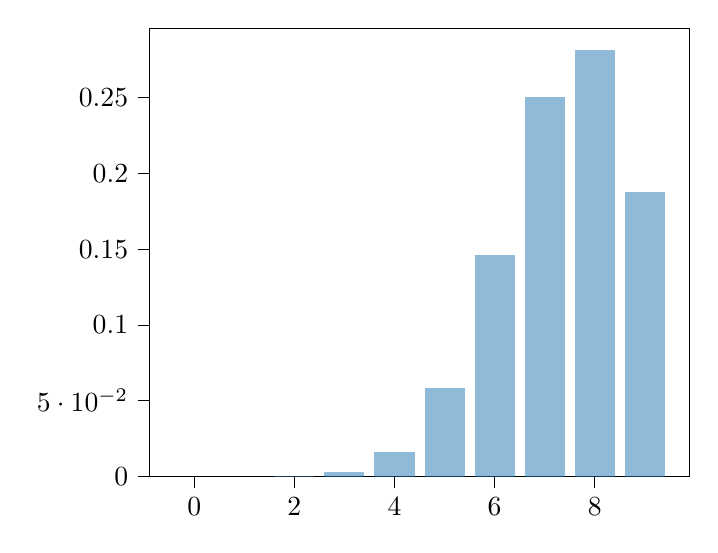
\begin{tikzpicture}

\definecolor{color0}{rgb}{0.12156862745098,0.466666666666667,0.705882352941177}

\begin{axis}[
tick align=outside,
tick pos=left,
x grid style={white!69.0196078431373!black},
xmin=-0.89, xmax=9.89,
xtick style={color=black},
y grid style={white!69.0196078431373!black},
ymin=0, ymax=0.295645952224731,
ytick style={color=black}
]
\draw[draw=none,fill=color0,fill opacity=0.5] (axis cs:-0.4,0) rectangle (axis cs:0.4,9.5367431640625e-07);
\draw[draw=none,fill=color0,fill opacity=0.5] (axis cs:0.6,0) rectangle (axis cs:1.4,2.86102294921875e-05);
\draw[draw=none,fill=color0,fill opacity=0.5] (axis cs:1.6,0) rectangle (axis cs:2.4,0.000386238098144531);
\draw[draw=none,fill=color0,fill opacity=0.5] (axis cs:2.6,0) rectangle (axis cs:3.4,0.00308990478515625);
\draw[draw=none,fill=color0,fill opacity=0.5] (axis cs:3.6,0) rectangle (axis cs:4.4,0.0162220001220703);
\draw[draw=none,fill=color0,fill opacity=0.5] (axis cs:4.6,0) rectangle (axis cs:5.4,0.0583992004394531);
\draw[draw=none,fill=color0,fill opacity=0.5] (axis cs:5.6,0) rectangle (axis cs:6.4,0.145998001098633);
\draw[draw=none,fill=color0,fill opacity=0.5] (axis cs:6.6,0) rectangle (axis cs:7.4,0.250282287597656);
\draw[draw=none,fill=color0,fill opacity=0.5] (axis cs:7.6,0) rectangle (axis cs:8.4,0.281567573547363);
\draw[draw=none,fill=color0,fill opacity=0.5] (axis cs:8.6,0) rectangle (axis cs:9.4,0.187711715698242);
\end{axis}

\end{tikzpicture}

% This file was created by tikzplotlib v0.9.8.
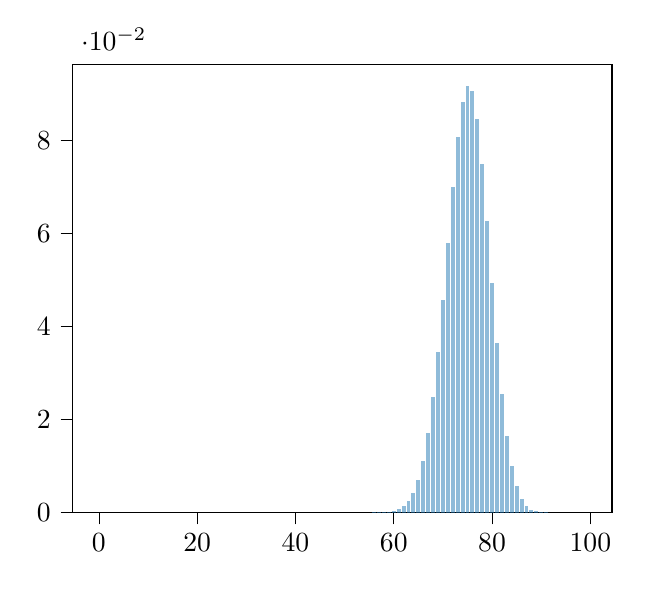
\begin{tikzpicture}

\definecolor{color0}{rgb}{0.12156862745098,0.466666666666667,0.705882352941177}

\begin{axis}[
tick align=outside,
tick pos=left,
x grid style={white!69.0196078431373!black},
xmin=-5.39, xmax=104.39,
xtick style={color=black},
y grid style={white!69.0196078431373!black},
ymin=0, ymax=0.0963896763551786,
ytick style={color=black}
]
\draw[draw=none,fill=color0,fill opacity=0.5] (axis cs:-0.4,0) rectangle (axis cs:0.4,6.22301527786114e-61);
\draw[draw=none,fill=color0,fill opacity=0.5] (axis cs:0.6,0) rectangle (axis cs:1.4,1.86690458335834e-58);
\draw[draw=none,fill=color0,fill opacity=0.5] (axis cs:1.6,0) rectangle (axis cs:2.4,2.77235330628714e-56);
\draw[draw=none,fill=color0,fill opacity=0.5] (axis cs:2.6,0) rectangle (axis cs:3.4,2.7169062401614e-54);
\draw[draw=none,fill=color0,fill opacity=0.5] (axis cs:3.6,0) rectangle (axis cs:4.4,1.97654928971742e-52);
\draw[draw=none,fill=color0,fill opacity=0.5] (axis cs:4.6,0) rectangle (axis cs:5.4,1.13849239087723e-50);
\draw[draw=none,fill=color0,fill opacity=0.5] (axis cs:5.6,0) rectangle (axis cs:6.4,5.40783885666685e-49);
\draw[draw=none,fill=color0,fill opacity=0.5] (axis cs:6.6,0) rectangle (axis cs:7.4,2.17858651082864e-47);
\draw[draw=none,fill=color0,fill opacity=0.5] (axis cs:7.6,0) rectangle (axis cs:8.4,7.5978204565149e-46);
\draw[draw=none,fill=color0,fill opacity=0.5] (axis cs:8.6,0) rectangle (axis cs:9.4,2.32999827333124e-44);
\draw[draw=none,fill=color0,fill opacity=0.5] (axis cs:9.6,0) rectangle (axis cs:10.4,6.36089528619427e-43);
\draw[draw=none,fill=color0,fill opacity=0.5] (axis cs:10.6,0) rectangle (axis cs:11.4,1.56131066115678e-41);
\draw[draw=none,fill=color0,fill opacity=0.5] (axis cs:11.6,0) rectangle (axis cs:12.4,3.47391622107383e-40);
\draw[draw=none,fill=color0,fill opacity=0.5] (axis cs:12.6,0) rectangle (axis cs:13.4,7.05472217202685e-39);
\draw[draw=none,fill=color0,fill opacity=0.5] (axis cs:13.6,0) rectangle (axis cs:14.4,1.31520177635643e-37);
\draw[draw=none,fill=color0,fill opacity=0.5] (axis cs:14.6,0) rectangle (axis cs:15.4,2.26214705533307e-36);
\draw[draw=none,fill=color0,fill opacity=0.5] (axis cs:15.6,0) rectangle (axis cs:16.4,3.60529686943707e-35);
\draw[draw=none,fill=color0,fill opacity=0.5] (axis cs:16.6,0) rectangle (axis cs:17.4,5.34432241822437e-34);
\draw[draw=none,fill=color0,fill opacity=0.5] (axis cs:17.6,0) rectangle (axis cs:18.4,7.39297934521038e-33);
\draw[draw=none,fill=color0,fill opacity=0.5] (axis cs:18.6,0) rectangle (axis cs:19.4,9.57196273116712e-32);
\draw[draw=none,fill=color0,fill opacity=0.5] (axis cs:19.6,0) rectangle (axis cs:20.4,1.1629934718368e-30);
\draw[draw=none,fill=color0,fill opacity=0.5] (axis cs:20.6,0) rectangle (axis cs:21.4,1.32913539638492e-29);
\draw[draw=none,fill=color0,fill opacity=0.5] (axis cs:21.6,0) rectangle (axis cs:22.4,1.4318413133783e-28);
\draw[draw=none,fill=color0,fill opacity=0.5] (axis cs:22.6,0) rectangle (axis cs:23.4,1.45674290143705e-27);
\draw[draw=none,fill=color0,fill opacity=0.5] (axis cs:23.6,0) rectangle (axis cs:24.4,1.40211504263316e-26);
\draw[draw=none,fill=color0,fill opacity=0.5] (axis cs:24.6,0) rectangle (axis cs:25.4,1.27872891888145e-25);
\draw[draw=none,fill=color0,fill opacity=0.5] (axis cs:25.6,0) rectangle (axis cs:26.4,1.1065923336474e-24);
\draw[draw=none,fill=color0,fill opacity=0.5] (axis cs:26.6,0) rectangle (axis cs:27.4,9.09864807665644e-24);
\draw[draw=none,fill=color0,fill opacity=0.5] (axis cs:27.6,0) rectangle (axis cs:28.4,7.11644260281343e-23);
\draw[draw=none,fill=color0,fill opacity=0.5] (axis cs:28.6,0) rectangle (axis cs:29.4,5.30052276623345e-22);
\draw[draw=none,fill=color0,fill opacity=0.5] (axis cs:29.6,0) rectangle (axis cs:30.4,3.76337116402575e-21);
\draw[draw=none,fill=color0,fill opacity=0.5] (axis cs:30.6,0) rectangle (axis cs:31.4,2.54938046595293e-20);
\draw[draw=none,fill=color0,fill opacity=0.5] (axis cs:31.6,0) rectangle (axis cs:32.4,1.6491304889133e-19);
\draw[draw=none,fill=color0,fill opacity=0.5] (axis cs:32.6,0) rectangle (axis cs:33.4,1.01946248405549e-18);
\draw[draw=none,fill=color0,fill opacity=0.5] (axis cs:33.6,0) rectangle (axis cs:34.4,6.02682233221042e-18);
\draw[draw=none,fill=color0,fill opacity=0.5] (axis cs:34.6,0) rectangle (axis cs:35.4,3.40945949079332e-17);
\draw[draw=none,fill=color0,fill opacity=0.5] (axis cs:35.6,0) rectangle (axis cs:36.4,1.84679055751305e-16);
\draw[draw=none,fill=color0,fill opacity=0.5] (axis cs:36.6,0) rectangle (axis cs:37.4,9.5833455957434e-16);
\draw[draw=none,fill=color0,fill opacity=0.5] (axis cs:37.6,0) rectangle (axis cs:38.4,4.76645346735658e-15);
\draw[draw=none,fill=color0,fill opacity=0.5] (axis cs:38.6,0) rectangle (axis cs:39.4,2.27323165366237e-14);
\draw[draw=none,fill=color0,fill opacity=0.5] (axis cs:39.6,0) rectangle (axis cs:40.4,1.04000348155053e-13);
\draw[draw=none,fill=color0,fill opacity=0.5] (axis cs:40.6,0) rectangle (axis cs:41.4,4.56586894339259e-13);
\draw[draw=none,fill=color0,fill opacity=0.5] (axis cs:41.6,0) rectangle (axis cs:42.4,1.92418762614402e-12);
\draw[draw=none,fill=color0,fill opacity=0.5] (axis cs:42.6,0) rectangle (axis cs:43.4,7.7862476034665e-12);
\draw[draw=none,fill=color0,fill opacity=0.5] (axis cs:43.6,0) rectangle (axis cs:44.4,3.02601895498357e-11);
\draw[draw=none,fill=color0,fill opacity=0.5] (axis cs:44.6,0) rectangle (axis cs:45.4,1.12971374319387e-10);
\draw[draw=none,fill=color0,fill opacity=0.5] (axis cs:45.6,0) rectangle (axis cs:46.4,4.05223407884757e-10);
\draw[draw=none,fill=color0,fill opacity=0.5] (axis cs:46.6,0) rectangle (axis cs:47.4,1.39672749100703e-09);
\draw[draw=none,fill=color0,fill opacity=0.5] (axis cs:47.6,0) rectangle (axis cs:48.4,4.6266598139608e-09);
\draw[draw=none,fill=color0,fill opacity=0.5] (axis cs:48.6,0) rectangle (axis cs:49.4,1.47297741015895e-08);
\draw[draw=none,fill=color0,fill opacity=0.5] (axis cs:49.6,0) rectangle (axis cs:50.4,4.50731087508638e-08);
\draw[draw=none,fill=color0,fill opacity=0.5] (axis cs:50.6,0) rectangle (axis cs:51.4,1.32567966914305e-07);
\draw[draw=none,fill=color0,fill opacity=0.5] (axis cs:51.6,0) rectangle (axis cs:52.4,3.74759444930825e-07);
\draw[draw=none,fill=color0,fill opacity=0.5] (axis cs:52.6,0) rectangle (axis cs:53.4,1.01821434094413e-06);
\draw[draw=none,fill=color0,fill opacity=0.5] (axis cs:53.6,0) rectangle (axis cs:54.4,2.65867077913189e-06);
\draw[draw=none,fill=color0,fill opacity=0.5] (axis cs:54.6,0) rectangle (axis cs:55.4,6.67084668218547e-06);
\draw[draw=none,fill=color0,fill opacity=0.5] (axis cs:55.6,0) rectangle (axis cs:56.4,1.60815053945542e-05);
\draw[draw=none,fill=color0,fill opacity=0.5] (axis cs:56.6,0) rectangle (axis cs:57.4,3.72413809137046e-05);
\draw[draw=none,fill=color0,fill opacity=0.5] (axis cs:57.6,0) rectangle (axis cs:58.4,8.2829967894274e-05);
\draw[draw=none,fill=color0,fill opacity=0.5] (axis cs:58.6,0) rectangle (axis cs:59.4,0.000176891117875907);
\draw[draw=none,fill=color0,fill opacity=0.5] (axis cs:59.6,0) rectangle (axis cs:60.4,0.00036262679164561);
\draw[draw=none,fill=color0,fill opacity=0.5] (axis cs:60.6,0) rectangle (axis cs:61.4,0.000713364180286445);
\draw[draw=none,fill=color0,fill opacity=0.5] (axis cs:61.6,0) rectangle (axis cs:62.4,0.00134618724344378);
\draw[draw=none,fill=color0,fill opacity=0.5] (axis cs:62.6,0) rectangle (axis cs:63.4,0.00243595786908874);
\draw[draw=none,fill=color0,fill opacity=0.5] (axis cs:63.6,0) rectangle (axis cs:64.4,0.00422486442920078);
\draw[draw=none,fill=color0,fill opacity=0.5] (axis cs:64.6,0) rectangle (axis cs:65.4,0.00701977474390283);
\draw[draw=none,fill=color0,fill opacity=0.5] (axis cs:65.6,0) rectangle (axis cs:66.4,0.011167823456209);
\draw[draw=none,fill=color0,fill opacity=0.5] (axis cs:66.6,0) rectangle (axis cs:67.4,0.0170017610825869);
\draw[draw=none,fill=color0,fill opacity=0.5] (axis cs:67.6,0) rectangle (axis cs:68.4,0.0247525639290604);
\draw[draw=none,fill=color0,fill opacity=0.5] (axis cs:68.6,0) rectangle (axis cs:69.4,0.0344383498143448);
\draw[draw=none,fill=color0,fill opacity=0.5] (axis cs:69.6,0) rectangle (axis cs:70.4,0.0457538076104867);
\draw[draw=none,fill=color0,fill opacity=0.5] (axis cs:70.6,0) rectangle (axis cs:71.4,0.0579977842949832);
\draw[draw=none,fill=color0,fill opacity=0.5] (axis cs:71.6,0) rectangle (axis cs:72.4,0.0700806560231046);
\draw[draw=none,fill=color0,fill opacity=0.5] (axis cs:72.6,0) rectangle (axis cs:73.4,0.0806407548759012);
\draw[draw=none,fill=color0,fill opacity=0.5] (axis cs:73.6,0) rectangle (axis cs:74.4,0.0882689343911892);
\draw[draw=none,fill=color0,fill opacity=0.5] (axis cs:74.6,0) rectangle (axis cs:75.4,0.0917996917668368);
\draw[draw=none,fill=color0,fill opacity=0.5] (axis cs:75.6,0) rectangle (axis cs:76.4,0.0905918010856942);
\draw[draw=none,fill=color0,fill opacity=0.5] (axis cs:76.6,0) rectangle (axis cs:77.4,0.0847092165996101);
\draw[draw=none,fill=color0,fill opacity=0.5] (axis cs:77.6,0) rectangle (axis cs:78.4,0.074935076222732);
\draw[draw=none,fill=color0,fill opacity=0.5] (axis cs:78.6,0) rectangle (axis cs:79.4,0.0626039877303837);
\draw[draw=none,fill=color0,fill opacity=0.5] (axis cs:79.6,0) rectangle (axis cs:80.4,0.0493006403376772);
\draw[draw=none,fill=color0,fill opacity=0.5] (axis cs:80.6,0) rectangle (axis cs:81.4,0.0365189928427239);
\draw[draw=none,fill=color0,fill opacity=0.5] (axis cs:81.6,0) rectangle (axis cs:82.4,0.0253851535614056);
\draw[draw=none,fill=color0,fill opacity=0.5] (axis cs:82.6,0) rectangle (axis cs:83.4,0.0165156420760952);
\draw[draw=none,fill=color0,fill opacity=0.5] (axis cs:83.6,0) rectangle (axis cs:84.4,0.0100273541176292);
\draw[draw=none,fill=color0,fill opacity=0.5] (axis cs:84.6,0) rectangle (axis cs:85.4,0.00566250585466122);
\draw[draw=none,fill=color0,fill opacity=0.5] (axis cs:85.6,0) rectangle (axis cs:86.4,0.00296293910999715);
\draw[draw=none,fill=color0,fill opacity=0.5] (axis cs:86.6,0) rectangle (axis cs:87.4,0.00143038439792966);
\draw[draw=none,fill=color0,fill opacity=0.5] (axis cs:87.6,0) rectangle (axis cs:88.4,0.000633920358173371);
\draw[draw=none,fill=color0,fill opacity=0.5] (axis cs:88.6,0) rectangle (axis cs:89.4,0.000256417223530802);
\draw[draw=none,fill=color0,fill opacity=0.5] (axis cs:89.6,0) rectangle (axis cs:90.4,9.40196486279606e-05);
\draw[draw=none,fill=color0,fill opacity=0.5] (axis cs:90.6,0) rectangle (axis cs:91.4,3.09954885586683e-05);
\draw[draw=none,fill=color0,fill opacity=0.5] (axis cs:91.6,0) rectangle (axis cs:92.4,9.09650207700049e-06);
\draw[draw=none,fill=color0,fill opacity=0.5] (axis cs:92.6,0) rectangle (axis cs:93.4,2.34748440696787e-06);
\draw[draw=none,fill=color0,fill opacity=0.5] (axis cs:93.6,0) rectangle (axis cs:94.4,5.24438005811971e-07);
\draw[draw=none,fill=color0,fill opacity=0.5] (axis cs:94.6,0) rectangle (axis cs:95.4,9.93672011012155e-08);
\draw[draw=none,fill=color0,fill opacity=0.5] (axis cs:95.6,0) rectangle (axis cs:96.4,1.55261251720649e-08);
\draw[draw=none,fill=color0,fill opacity=0.5] (axis cs:96.6,0) rectangle (axis cs:97.4,1.92075775324514e-09);
\draw[draw=none,fill=color0,fill opacity=0.5] (axis cs:97.6,0) rectangle (axis cs:98.4,1.76396120195983e-10);
\draw[draw=none,fill=color0,fill opacity=0.5] (axis cs:98.6,0) rectangle (axis cs:99.4,1.06906739512717e-11);
\end{axis}

\end{tikzpicture}

\end{center}


Au début de ce chapitre, nous avons décrit des situations probabilistes en définissant
proprement un univers $\Omega$ ainsi qu'une probabilité $\mathbb{P}$ sur $\Omega$.
Mais en avançant dans les exercices, nous nous sommes éloignés
de l'univers $\Omega$ pour décrire désormais notre expérience à l'aide de variables aléatoires.
C'est ce que nous ferons de plus en plus. La description de notre problème probabiliste
se fera par la donnée d'une ou plusieurs variables aléatoires dont nous donnerons les
lois, plutôt que de nous concentrer sur l'espace probabilisé $(\Omega,\mathbb{P})$. Cette
abstraction nous sera très utile. Par exemple, si on lance un dé à 6 faces, on a envie
de choisir $\Omega_1=\intere{1}{6}$ muni de la probabilité uniforme. Mais si on lance
deux fois le dé, l'univers $\Omega_2=\intere{1}{6}^2$ muni de la loi uniforme semble
plus approprié. Toute probabilité d'un évènement faisant intervenir les deux lancers de
dés doit être calculée dans le cadre de l'univers $\Omega_2$. Cependant $\Omega_1$ nous suffit
si on s'intéresse uniquement au premier lancer. Pour autant, doit-on changer d'univers à chaque fois
qu'on change de question~? La réponse des probabilistes à ce problème consiste à négliger
une bonne fois pour toutes l'univers $\Omega$. Par exemple, si un exercice vous met dans la
situation \og On lance un dé à 6 faces et on note $X$ la face obtenue \fg, vous pouvez
affirmer que $X$ est une variable aléatoire suivant la loi uniforme sur $\intere{1}{6}$
sans évoquer l'espace probabilisé $(\Omega,\mathbb{P})$.\\

Cependant, les mathématiciens se demandent souvent si les objets qu'ils manipulent existent bien.
En prépa, c'est un problème que nous pourrons le plus souvent ignorer. Mais, lorsque l'on souhaite
travailler avec la rigueur que nous permettent les mathématiques, il est important de démontrer que
les espaces probabilisés dont nous parlons existent bien. De nombreux théorèmes, qui ne sont pas
au programme de prépa, nous permettent de
justifier l'existence de tels espaces. Par exemple, si $E$ est un ensemble fini et $(p_x)_{x\in E}$ est
une distribution de probabilités sur $E$, on peut montrer qu'il existe bien un espace probabilisé
$(\Omega,\mathbb{P})$ et une variable aléatoire $X:\Omega\to E$ telle que
\[\forall x\in E\qsep \mathbb{P}(X=x)=p_x.\]

\section{Dépendance des évènements}

\subsection{Probabilité conditionnelle}

On se donne une expérience aléatoire associée à un espace probabilisé $(\Omega,\mathbb{P})$.
Soit $A$ et $B$ deux évènements tels que $\mathbb{P}(B)>0$. Si on réalise $n$ fois cette
expérience aléatoire et qu'on compte le nombre de fois $n_B$ où l'évènement $B$ a été réalisé
ainsi que le nombre de fois $n_{A\cap B}$ parmi ces réalisations où l'évènement $A$ a aussi
été réalisé, alors
\[\frac{n_{A\cap B}}{n_B}=\frac{n_{A\cap B}}{n}\cdot\frac{n}{n_B}
  \tendvers{n}{+\infty} \frac{\mathbb{P}(A\cap B)}{\mathbb{P}(B)}.\]
On appelle ce nombre, probabilité de $A$ sachant $B$.

\begin{definition}
Soit $B\in\mathcal{P}(\Omega)$ un évènement
de probabilité non nulle. Pour tout évènement $A\in\mathcal{P}(\Omega)$, on appelle
\emph{probabilité de $A$ sachant $B$} le nombre
\[\mathbb{P}(A|B)=\frac{\mathbb{P}(A\cap B)}{\mathbb{P}(B)}.\]
\end{definition}

\begin{proposition}
Soit $B\in\mathcal{P}(\Omega)$ un évènement
de probabilité non nulle. Alors l'application
\[\dspappli{\mathbb{P}_B}{\mathcal{P}(\Omega)}{\interf{0}{1}}{A}{\mathbb{P}(A|B)}\]
est une probabilité sur $\Omega$.
\end{proposition}

\begin{remarqueUnique}
\remarque Attention, bien qu'on écrive $\mathbb{P}(A|B)$, $A|B$ n'est pas un évènement.
  La notation $\mathbb{P}_B(A)$ protège contre cette erreur.
\end{remarqueUnique}

\subsection{Formule des probabilités totales}

\begin{proposition}[nom={Formule des probabilités totales}]
Soit $(A_1,\ldots,A_n)$ un système complet d'évènements. Alors, pour tout évènement $B$
\[\mathbb{P}(B)=\sum_{i=1}^n \mathbb{P}(A_i)\mathbb{P}(B|A_i).\]
\end{proposition}

\begin{remarques}
\remarque Dans cette formule, par convention, on remplacera
  $\mathbb{P}(A_i)\mathbb{P}(B|A_i)$ par $0$ lorsque $\mathbb{P}(A_i)=0$.
\remarque C'est cette formule qui se cache derrière les arbres de probabilité
  utilisés dans le secondaire. Afin d'aborder des exercices plus complexes,
  il est important de ne plus recourir à ces arbres et d'utiliser directement la formule
  des probabilités totales.
\end{remarques}
\vspace{1ex}
\begin{exoUnique}
\exo Une urne contient $n\in\Ns$ boules noires et $b\in\Ns$ boules blanches. On tire deux boules
  successivement sans remise. Avec quelle probabilité la deuxième boule tirée est-elle
  blanche~?
\begin{sol}
$B_1\defeq$\og La première boule tirée est blanche\fg et 
$B_2\defeq$\og La seconde boule tirée est blanche\fg. Alors $\mathbb{P}(B_1)=b/(n+b)$ et $\mathbb{P}(B_2|B_1)=(b-1)/(n+b-1)$,
$\mathbb{P}(B_2|N_1)=b/(n+b-1)$, donc $\mathbb{P}(B_2)=\frac{b}{n+b}\frac{b-1}{n+b-1}+\frac{n}{n+b}\frac{b}{n+b-1}=\frac{b}{n+b}$.
On remarque que $B_1$ et $B_2$ sont équiprobables.
\end{sol}
\end{exoUnique}

\begin{proposition}[nom={Formule des probabilités composées}]
  Soit $A_1,\ldots,A_n$ des évènements tels que $\mathbb{P}(A_1\cap\ldots\cap A_{n-1})>0$.
  Alors
  \[\mathbb{P}(A_1\cap\ldots\cap A_n)=
    \mathbb{P}(A_1)\mathbb{P}(A_2|A_1)\mathbb{P}(A_3|A_1\cap A_2)
    \cdots \mathbb{P}(A_n|A_1\cap\ldots\cap A_{n-1}).\]
\end{proposition}
  
\begin{exos}
\exo Une urne contient $2n$ boules dont $n$ noires et $n$ blanches. On en tire 3 boules successivement. Avec quelle
  probabilité les tire-t-on dans l'ordre \og noire, blanche, noire \fg si les tirages se font avec remise~? Et s'ils
  se font sans remise~?
  \begin{sol}
  Avec remise, $1/8$, sans remise $n/(4(2n-1))$.
  \end{sol}
% \exo Un commerçant met en vente 50 tickets d'un jeu dont exactement 3 sont gagnants. Je lui achète 6 tickets.
%   Avec quelle probabilité en ai-je acheté au moins un gagnant~?
\exo Une urne contient initialement une boule blanche et une boule noire. On y effectue
  $m$ tirages successifs. À chaque tirage, la boule est choisie avec une probabilité
  uniforme sur toutes les boules présentes. Avant le tirage suivant, on replace dans l’urne
  la boule tirée et on ajoute une boule supplémentaire de la même couleur. Pour tout
  $n\in\intere{1}{m}$, on désigne par $X_n$ le nombre de boules blanches obtenues au cours
  des $n$ premiers tirages.
  \begin{questions}
  \question Déterminer la loi de $X_1$, la loi de $X_2$.
  \question Calculer $\mathbb{P}(X_n = 0)$ et $\mathbb{P}(X_n = n)$.
  \question En déduire, par récurrence, la loi de $X_n$.
  \end{questions}
\begin{sol}
\begin{questions}
\question $\mathbb{P}(X_1=0)=1/2$, $\mathbb{P}(X_1=1)=1/2$. $\mathbb{P}(X_2=0)=1/3$, $\mathbb{P}(X_2=1)=$.
\end{questions}
$\mathbb{P}(X_n=k)=1/(n+1)$.
\end{sol}
\end{exos}

\subsection{Formule de \nom{Bayes}}

\begin{proposition}[nom={Formule de \nom{Bayes}}]
Soit $A$ et $B$ deux évènements de probabilité non nulle. Alors
\[\mathbb{P}(A|B)=\frac{\mathbb{P}(A)}{\mathbb{P}(B)}\cdot\mathbb{P}(B|A).\]
\end{proposition}

\begin{remarqueUnique}
\remarque Si de plus $(C_1,\ldots,C_n)$ forme un système complet d'évènements
  \[\mathbb{P}(A|B)=\frac{\mathbb{P}(A)}{%
    \sum_{i=1}^n \mathbb{P}(C_i)\mathbb{P}(B|C_i)}%
    \cdot\mathbb{P}(B|A).\]
\end{remarqueUnique}

\begin{exoUnique}
\exo Un laboratoire pharmaceutique indique pour un test permettant de détecter une maladie,
  sa sensibilité $\alpha$ qui est la probabilité que le test soit positif si le sujet est
  malade, et sa spécificité $\beta$ qui est la probabilité que le test soit négatif si le
  sujet est sain. Sachant qu'en moyenne il y a un malade sur 1000 personnes,
  calculer la probabilité pour que vous soyez un sujet sain alors que votre test est positif.
  Faites une application numérique pour $\alpha\defeq 98\%$ et $\beta\defeq 97\%$. 
   \begin{sol}
   $$\pr{S | +} = \frac{\pr{S}}{\pr{+}} \pr{+ |S}= \frac{ \frac{999}{1000}}{\pr{+}} \left( 1 - \pr{- |S} \right)= \frac{ \frac{999}{1000}}{\pr{+}} \left( 1 - \beta \right) \quad \textbf{Bayes}$$
   $$\pr{+}=\pr{+ | M} \pr{M} + \pr{+ | S} \pr{S} = \alpha \frac 1{1000} + (1-
   \beta) \frac{999}{1000} \quad \textbf{probas totales}$$
   donc $\boxed{\pr{S | +} = \frac 1{1+ \frac{\alpha}{999(1-\beta)}} \simeq
   96,8 \%}$. C'est donc très mauvais ! Si $\beta$ est très proche de $1$ alors
   $\pr{S | +}$ est proche de $0$ donc le test devient fiable \dots
   \end{sol}
\end{exoUnique}

\subsection{Indépendance}

\begin{definition}
On dit que deux évènements
$A,B\in\mathcal{P}(\Omega)$ sont \emph{indépendants} lorsque
\[\mathbb{P}(A\cap B)=\mathbb{P}(A)\mathbb{P}(B).\]
\end{definition}

\begin{remarques}
\remarque Si $A$ et $B$ sont deux évènements tels que $B$ est de probabilité non nulle,
  alors $A$ et $B$ sont indépendants si et seulement si $\mathbb{P}(A|B)=\mathbb{P}(A)$.
\remarque Il est important de ne pas confondre les notions d'incompatibilité et d'indépendance.
  Notons d'ailleurs que la notion d'incompatibilité ne dépend pas de la loi de probabilité
  utilisée alors que la notion d'indépendance en dépend.
\end{remarques}

\begin{proposition}
Soit $A$ et $B$ deux évènements indépendants. Alors $A$ et $\bar{B}$ sont indépendants.
\end{proposition}

\begin{remarqueUnique}
\remarque On en déduit que si $A$ et $B$ sont indépendants, il en est de même pour $\bar{A}$ et $B$,
 ainsi que pour $\bar{A}$ et $\bar{B}$.
\end{remarqueUnique}

\begin{definition}
On dit que les évènements
$A_1,\ldots,A_n\in\mathcal{P}(\Omega)$ sont \emph{mutuellement indépendants} lorsque,
quel que soit $I\subset\intere{1}{n}$
\[\mathbb{P}\p{\bigcap_{i\in I} A_i}=\prod_{i\in I} \mathbb{P}(A_i).\]
\end{definition}

\begin{remarques}
\remarque Si $A_1,\ldots,A_n\in\mathcal{P}(\Omega)$ sont mutuellement indépendants, alors
  ils sont deux à deux indépendants. Autrement dit
  \[\forall i,j\in\intere{1}{n}\qsep i\neq j \quad\implique\quad \mathbb{P}(A_i\cap A_j)
    =\mathbb{P}(A_i)\mathbb{P}(A_j).\]
  Cependant, comme le montre le prochain exercice, des évènements peuvent être deux à deux
  indépendants sans être mutuellement indépendants.
\remarque Si $A_1,\ldots,A_n\in\mathcal{P}(\Omega)$ sont mutuellement indépendants, alors
  $B_1\in\{A_1,\bar{A_1}\},\ldots,B_n\in\{A_n,\bar{A_n}\}$ sont mutuellement indépendants.
\end{remarques}

\begin{exoUnique}
\exo On lance successivement deux dés équilibrés. On modélise cela en prenant
  $\Omega\defeq\intere{1}{6}^2$ que l'on munit de la probabilité uniforme.
  On considère les évènements suivants~:
  \begin{itemize}
  \item $A\defeq$ \og Le premier dé est pair \fg.
  \item $B\defeq$ \og Le second dé est impair \fg.
  \item $C\defeq$ \og La somme des deux dés est paire \fg.
  \end{itemize}
  Sont-ils deux à deux indépendants~? Sont-ils mutuellement indépendants~?
  % \begin{sol}
  % Ces trois évènements sont de proba $1/2$ (pour le dernier, on peut le voir en énumérant tous les cas (dans un tableau ?)). On montre ensuite qu'ils sont deux à deux indépendants en calculant les probabilités des intersections. En revanche, $\pr{A\cap B\cap C}=0$ donc ils ne sont pas mutuellement indépendants.
  % \end{sol}
  % \exo Soit $n \geq 2$. On lance $n$ fois une pièce équilibrée. On note $A$ l'évènement \og toutes les pièces tombent du même côté \fg et $B$ l'évènement \og on obtient au plus un {\it face}\fg. $A$ et $B$ sont-ils indépendants ?
  % \begin{sol}
  % On a $\pr{A}=2\p{\frac{1}{2}}^n=\p{\frac{1}{2}}^{n-1}$ et $B$ est l'union des évènements incompatibles "on fait que des piles" et "on fait exactement un face" $\pr{B}=\p{\frac{1}{2}}^n+n\p{\frac{1}{2}}^n$. On a donc $\pr{A}\pr{B}=\frac{2(n+1)}{2^{2n}}$.
  % $A\cap B$ est l'évènement "on fait que des piles" (car $n\geq 2$) de probabilité $\pr{A\cap B}=\p{\frac{1}{2}}^n$. 
  % Les évènements $A$ et $B$ ne sont donc pas indépendants.
  % \end{sol}
\end{exoUnique}

\begin{definition}
\begin{itemize}
\item On dit que deux variables aléatoires $X:\Omega\to E$ et $Y:\Omega\to F$ sont
  \emph{indépendantes} lorsque quelles que soient les parties $A\in\mathcal{P}(E)$ et
  $B\in\mathcal{P}(F)$, les évènements $(X\in A)$ et $(Y\in B)$ sont
  indépendants.
\item On dit que $n$ variables aléatoires $X_1:\Omega\to E_1,\ldots,X_n:\Omega\to E_n$ sont
\emph{mutuellement indépendantes} lorsque quelles que soient les parties
$A_1\in\mathcal{P}(E_1),\ldots,A_n\in\mathcal{P}(E_n)$, les évènements
$(X_1\in A_1),\ldots,(X_n\in A_n)\in\mathcal{P}(\Omega)$ sont mutuellement indépendants.
\end{itemize}
\end{definition}

\begin{remarques}
\remarque Si $X$ et $Y$ sont indépendantes, on note $X \indep Y$.
\remarque Si $X_1,\ldots,X_n$ sont mutuellement indépendantes, alors elles sont
  deux à deux indépendantes. Cependant, la réciproque est fausse. Lorsqu'on parle de variables aléatoires
  indépendantes sans plus de précision, il faut comprendre que les variables aléatoires sont
  mutuellement indépendantes.
\end{remarques}

\begin{proposition}
Soit $X_1:\Omega\to E_1,\ldots,X_n:\Omega\to E_n$, $n$ variables aléatoires. Alors, elles sont mutuellement
indépendantes si et seulement si
\[\forall (x_1,\ldots,x_n)\in X_1(\Omega)\times\cdots\times X_n(\Omega)\qsep
  \mathbb{P}((X_1=x_1)\cap\cdots\cap(X_n=x_n))=\mathbb{P}(X=x_1)\cdots\mathbb{P}(X_n=x_n).\] 
\end{proposition}

\begin{remarqueUnique}
\remarque Soit $A_1,\ldots,A_n\in\mathbb{P}(\Omega)$. Alors $A_1,\ldots,A_n$ sont mutuellement
  indépendants si et seulement si les variables aléatoires $\mathds{1}_{A_1},\ldots,\mathds{1}_{A_n}$
  sont mutuellement indépendantes.
\end{remarqueUnique}

\begin{exoUnique}
\exo Soit $X,Y,Z$ trois variables aléatoires mutuellement
  indépendantes qui suivent la même loi de
  \nom{Bernoulli} de paramètre $p\in[0,1]$. Donner une condition nécessaire et
  suffisante sur $p$ pour que les évènements $(X=Y)$ et $(Y=Z)$ soient
  indépendants.
% \begin{reponse}
% On note $A=(X=Y)$ et $B=(Y=Z)$. Alors
% $$\pr{A}=\pr{\p{X=0 \cap Y=0} \cup \p{X=1 \cap Y=1}} =\pr{X=0}\pr{Y=0} + \pr{X=1} \pr{Y=1}$$
% puisque les évènements $(X=0 \cap Y=0)$ et $(X=1 \cap Y=1)$ sont incompatibles et les évènements $(X=0)$ et $(Y=0)$ sont indépendants. On a donc $\pr{A}=p^2+q^2$. De même $\pr{B}=p^2+q^2$ et $\pr{A \cap B }=p^3+q^3$. 
% Mais $(p^2+q^2)^2-(p^3+q^3)=p(p-1)(2p-1)^2$ donc \fbox{il y a indépendance ssi $p=0,1$ ou $\frac 12$}.
% \end{reponse}
\end{exoUnique}

\begin{proposition}[nom={Lemme des coalitions}]
\begin{itemize}
\item 
Soit $X_1:\Omega\to E_1,\ldots,X_n:\Omega\to E_n$, des variables aléatoires mutuellement
indépendantes et
\[f:E_1\times\cdots\times E_m\to F,\qquad g:E_{m+1}\times\cdots\times E_n\to G\]
deux fonctions. Alors, les variables aléatoires $f(X_1,\ldots,X_m):\Omega\to F$ et
$g(X_{m+1},\ldots,X_n):\Omega\to G$ sont indépendantes. 
\item Soit $A_1,\ldots,A_n$ des évènements mutuellement indépendants. Si $B$ est un
 évènement défini à partir des évènements $A_1,\ldots,A_m$ et $C$ est un évènement
 défini à partir des évènements $A_{m+1},\ldots,A_n$, alors $B$ et $C$ sont
 indépendants.
\end{itemize}
\end{proposition}

\begin{remarques}
\remarque Cet énoncé se généralise facilement à un nombre fini de coalitions et nous
  assure que les variables aléatoires et les évènements obtenus sont mutuellement
  indépendants.
\remarque Supposons que l'on lance $n$ fois une pièce et que les $n$ lancers sont
  indépendants. Si $p,q\in\N$ sont tels que $p+q=n$, alors la variable aléatoire $Y$
  donnant le nombre de pile lors des $p$ premiers lancers est indépendante de la
  variable aléatoire $Z$ donnant le nombre de pile lors des $q$ derniers lancers.
% \remarque Si $E$ et $F$ sont deux ensembles finis, $(p_x)_{x\in E}$ est une distribution
%   de probabilités sur $E$ et $(q_y)_{y\in F}$ est une distribution de probabilités sur $F$,
%   on peut montrer qu'il existe un espace probabilisé $(\Omega,\mathbb{P})$ et deux
%   variables aléatoires indépendantes $X:\Omega\to E$ et $Y:\Omega\to F$ telles que
%   \[\cro{\forall x\in E\qsep \mathbb{P}(X=x)=p_x} \quad\et\quad \cro{\forall y\in F\qsep \mathbb{P}(Y=y)=q_y}.\]
%   Bien entendu, cette proposition se généralise à un nombre fini d'ensembles finis
%   $E_1,\ldots,E_n$ et permet de justifier l'existence d'un espace probabilisé
%   $(\Omega,\mathbb{P})$ et de variables aléatoires
%   $X_1:\Omega\to E_1,\ldots,X_n:\Omega\to E_n$ mutuellement indépendantes ayant une
%   loi donnée.
\end{remarques}

\begin{exoUnique}
\exo Soit $X_1,\ldots,X_n:\Omega\to\R$ une famille de variables aléatoires mutuellement
  indépendantes suivant toutes une loi de \nom{Rademacher}. Pour tout $i\in\intere{1}{n-1}$,
  on pose $Y_i\defeq X_i X_{i+1}$.
  \begin{questions}
  \question Montrer que les variables $Y_1,\ldots,Y_{n-1}$ sont deux à deux indépendantes.
  \question Sont-elles mutuellement indépendantes~?
  \end{questions}
\end{exoUnique}



\subsection{Loi d'une somme}

\begin{proposition}
Soit $X,Y:\Omega\to\N$ deux variables aléatoires indépendantes. Alors
\[\forall n\in\N\qsep\mathbb{P}(X+Y=n)=\sum_{k=0}^n  \mathbb{P}(X=k) \mathbb{P}(Y=n-k).\]
\end{proposition}

\begin{remarqueUnique}
\remarque Plus généralement, si $X,Y:\Omega\to\N$ sont deux variables dont on
  ne fait aucune hypothèse d'indépendance
  \[\forall n\in\N\qsep \mathbb{P}(X+Y=n)=\sum_{k=0}^n  \mathbb{P}((X=k)\cap(Y=n-k)).\] 
\end{remarqueUnique}

\begin{proposition}
Soit $X,Y:\Omega\to\N$ deux variables aléatoires indépendantes. On suppose qu'il existe
$p\in[0,1]$ et $n,m\in\N$ tels que $X\sim\mathcal{B}(n,p)$ et $Y\sim\mathcal{B}(m,p)$. Alors
$X+Y\sim\mathcal{B}(n+m,p)$.
\end{proposition}

\begin{proposition}
Soit $X_1,\ldots,X_n:\Omega\to\ens{0,1}$ des variables de \nom{Bernoulli} mutuellement indépendantes de
même paramètre $p\in[0,1]$.  Alors
\[X_1+\cdots+X_n \sim \mathcal{B}(n,p).\]
\end{proposition}

\begin{exoUnique}
\exo Deux joueurs lancent une pièce de monnaie équilibrée $n$ fois chacun. Calculer la
  probabilité qu'ils obtiennent le même nombre de fois pile. En déterminer un équivalent
  lorsque $n$ tend vers $+\infty$.
\begin{sol}
Soient $X$ et $Y$ les variables aléatoires discrètes qui représentent le nombre de piles obtenus par chacun des joueurs au cours des $n$ lancers. Les variables $X$ et $Y$ sont indépendantes et suivent des loi binomiales ${\cal B}(n, 1/2)$.
\[\pr{Y=k} = \sum\limits_{k=0}^n \left( \binom{n}{k} \left( \frac 12 \right)^k
  \left( \frac 12 \right)^{n-k} \right)^2\]
\[= \frac 1{4^n} \sum\limits_{k=0}^n \binom{n}{k} ^2 = \frac 1{4^n} \binom{2n}{n}
\sim \frac{1}{\sqrt{\pi n}}\]
\end{sol}
\end{exoUnique}

%END_BOOK
\end{document}


